\documentclass{article}
\usepackage[T1]{fontenc}
\usepackage{hyperref}
\usepackage{amsmath}
\usepackage[utf8]{inputenc}
\usepackage[polish]{babel}
\usepackage{graphicx}
\usepackage{amsfonts}
\usepackage{placeins}


\setlength{\textheight}{21cm}

\title{{\bf Zadanie nr 3 - Splot, filtracja i korelacja sygnałów}\linebreak
Cyfrowe Przetwarzanie Sygnałów}
\author{Dominik Gałkowski, 247659 \and Jan Śladowski, 247806}
\date{20.05.2025}

\begin{document}
\clearpage\maketitle
\thispagestyle{empty}
\newpage
\setcounter{page}{1}
\section{Cel zadania}

Celem zadania jest zapoznanie się z operacjami splotu dyskretnego i korelacji
dyskretnej, zaimplementowaniu tych operacji oraz wykorzystaniu ich przy
tworzeniu i zapoznawaniu sie z filtrami o skończonej odpowiedzi impulsowej.
\section{Wstęp teoretyczny}

Jest to usprawniony program z zadania 1 oraz 2, dostosowany do instrukcji z zadania trzeciego ~\cite{instrukcja}. \\

Zadanie polegało na zaimplementowaniu algorytmu, który umożliwi projektowanie filtrów dolnoprzepustowych żądanej liczbie współczynnikowi żądanej częstotliwości obcięcia z wykorzystaniem okien:
\begin{itemize}
	\item (O1) okno Hamminga,
	\item (O2) okno Hanninga,
	\item (O3) okno Blackmana,
	\item (O4) okno prostokątne,
\end{itemize}

Ponadto, w ramach realizacji ćwiczenia należało zaprojektować filtr z możliwością wyboru funkcji okna i parametrów filtru jak wyżej:
\begin{itemize}
	\item (F1) pasmowoprzepustowy,
	\item (F2) górnoprzepustowy,
\end{itemize} 

Należało także zaimplementować operacje filtracji podstawiając odpowiedz impulsowa filtru do wzoru na splot, zademonstrować efekt filtracji na arbitralnie wybranych sygnałach testowych. Ponadto, wymagana jest implementacja operacji korelacji dla dowolnych dwóch sygnałow dyskretnych o arbitralnie podanych ilościach próbek wzbogacone o dwa obligatoryjne warianty:
\begin{itemize}
	\item implementacje bezpośrednia,
	\item implementacje z użyciem splotu,
\end{itemize}

Celem części zadania związanej z zastosowaniem analizy korelacyjnej (pomiaru długości) była symulacja działania korelacyjnego czujnika odległości. 


\section{Materiały i metody} 
    \subsection{Splot i korelacja sygnałów dyskretnych} {
        Pojedynczy eksperyment składał się z kilku kroków. Najpierw wygenerowano wybrane sygnały
        ciągłe (wykorzystano funkcję sin, kwadratową i trójkątną), następnie spróbkowano je z
        ustaloną częstotliwości i na wynikach próbkowania przeprowadzono operację splotu lub
        korelacji.
    }

    \subsection{Filtracja sygnałów dyskretnych} \label{metody:filtracja}{
            W każdym eksperymencie mającym na celu prezentację procesu filtrowania wykorzystany
            został inny filtr, który uprzednio wygenerowano wykorzystując wybrane parametry. Sygnał
            filtrowany natomiast wykorzystano ten sam, dla wszystkich eksperymentów. Jest to
            suma dwóch sygnałów sinusoidalnych $s_1$ i $s_2$ o następujących parametrach:
            \begin{itemize}
                \item częstotliwość $f_{s_1} = 3Hz$
                \item amplituda $A_{s_1} = 2$
                \item częstotliwość $f_{s_2} = 20Hz$
                \item amplituda $A_{s_2} = 0.5$
                \item czas trwania $1s$
                \item częstotliwość próbkowania $f_s = 400Hz$
            \end{itemize}
            \begin{figure}[h!]
                \centering
                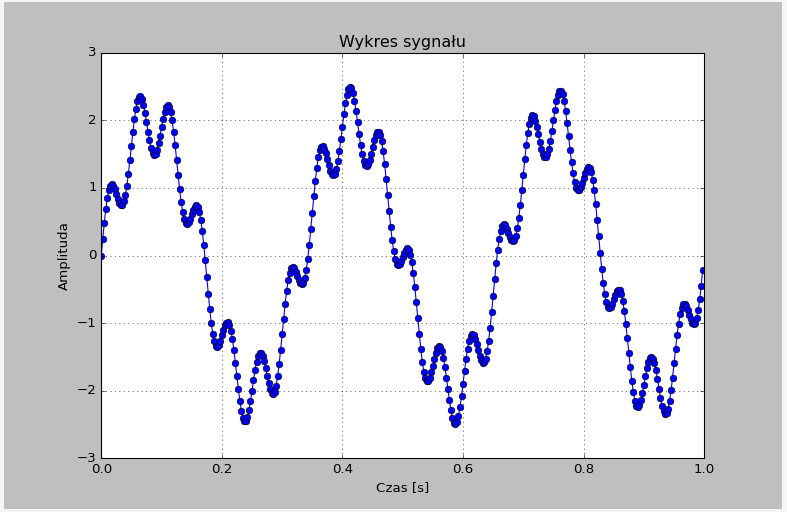
\includegraphics[width=0.7\textwidth]{img/sig.png}
                \caption{Sygnał filtrowany} \label{wykres:filtrowany}
            \end{figure}
            Każdorazowo po wygenerowaniu filtru obliczony został jego splot z sygnałem
            filtrowanym. Dla każdego eksperymentu zaprezentowano parametry i typ generowanego
            filtru, sam filtr oraz wynik splotu.
        }
        
        \subsection{Wykorzystanie analizy korelacyjnej do pomiaru odległości} {
            W przypadku wykorzystania analizy korelacyjnej do pomiaru odległości wykorzystano
            niezależną funkcjonalność aplikacji, jaką jest symulator korelacyjnego czujnika
            odległości. Każdy eksperyment wykonany został poprzez jednokrotne uruchomienie
            symulatora. Udokumentowane zostały parametry wejściowe i parametry wyjściowe z
            kilku chwil czasu. Wykorzystane zostały następujące oznaczenia parametrów
            wejściowych:
            \begin{itemize}
                \item $V_s[m/s]$ - prędkość sygnału w ośrodku
                \item $V_p[m/s]$ - prędkość przedmiotu
                \item $T_s[s]$ - okres sygnału sondującego
                \item $f_s[Hz]$ - częstotliwość próbkowania czujnika odległości
                \item $l$ - długość bufora czujnika odległości
            \end{itemize}
            Okres raportowania dla wszystkich ekspeymentów wysnosi 0.5s, natomiast jednostka czasowa wynosi 0.1s.

            Wykorzystane zostały następujące oznaczenia parametrów wyjściowych:
            \begin{itemize}
                \item $t[s]$ - chwila czasu
                \item $d_r[m]$ - odległość rzeczywista do przedmiotu
                \item $d_m[s]$ - odległość obliczona przez czujnik odległości
            \end{itemize}
        }
\newpage
\section{Eksperymenty i wyniki} {
    \subsection{Splot i korelacja sygnałów dyskretnych} 
    \subsubsection{Splot sygnałów sinusoidalnych} \label{eksperyment:splot1}{

                \begin{table}[h!]
                    \centering
                    \begin{tabular}{|l|l|l|l|l|}
                        \hline
                        Amplitiuda & Czas początkowy & \shortstack{Czas trwania \\ sygnału} & \shortstack{Okres \\ podstawowy} & \shortstack{Częstotliwość\\ próbkowania}   \\ \hline
                        1 & 0s & 3s & 1 & 100           \\ \hline
                    \end{tabular}
                    \caption{Parametry wejściowe dla sygnału nr 1}
                \end{table}
                \begin{figure}[h!]
                    \centering
                    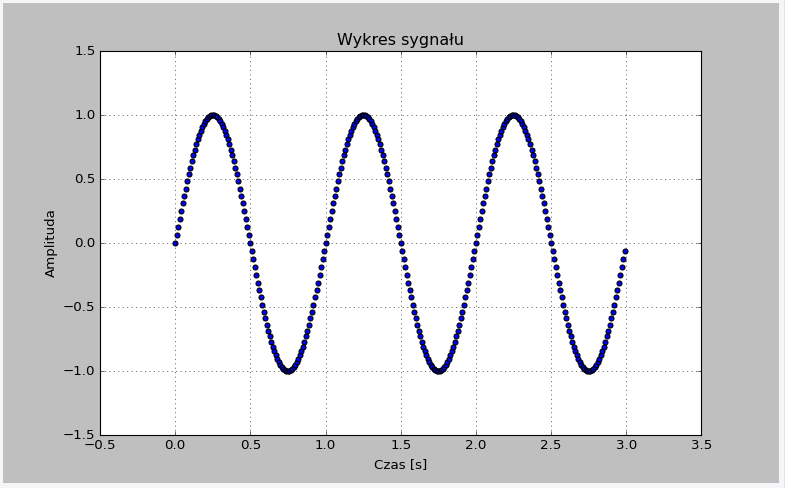
\includegraphics[width=0.7\textwidth]{img/splot1.png}
                    \caption{Wykres sygnału numer 1}
                \end{figure}

                \begin{table}[h!]
                    \centering
                    \begin{tabular}{|l|l|l|l|l|}
                        \hline
                        Amplitiuda & Czas początkowy & \shortstack{Czas trwania \\ sygnału} & \shortstack{Okres \\ podstawowy} & \shortstack{Częstotliwość\\ próbkowania}   \\ \hline
                        1 & 2s & 3s & 1 & 100           \\ \hline
                    \end{tabular}
                    \caption{Parametry wejściowe dla sygnału nr 2}
                \end{table}
                \begin{figure}[h!]
                    \centering
                    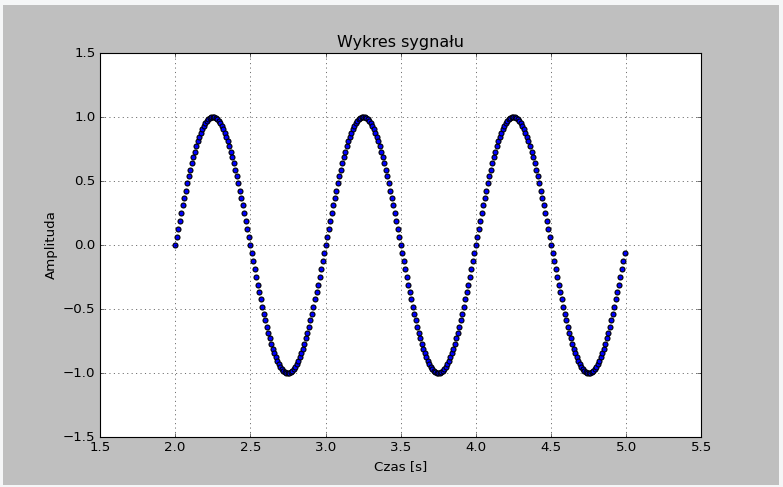
\includegraphics[width=0.7\textwidth]{img/splot2.png}
                    \caption{Wykres sygnału numer 2}
                \end{figure}

                \begin{figure}[h!]
                    \centering
                    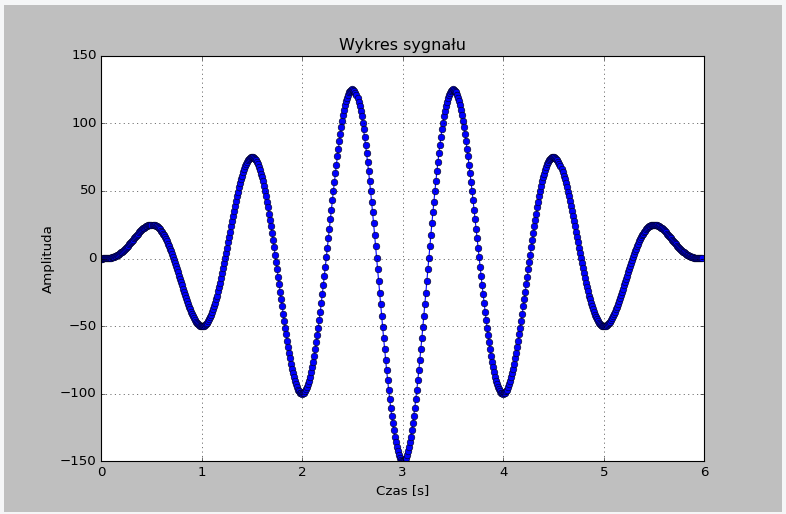
\includegraphics[width=0.7\textwidth]{img/splot3.png}
                    \caption{Wykres sygnału po operacji splotu}
                \end{figure}
            }
            \FloatBarrier
        \subsubsection{Splot sygnałów sinsoidalnego oraz sinusoidalnego wyprostowanego
            jednopołówkowo} \label{eksperyment:splot2}{

            \begin{table}[h!]
                \centering
                \begin{tabular}{|l|l|l|l|l|}
                    \hline
                    Amplitiuda & Czas początkowy & \shortstack{Czas trwania \\ sygnału} & \shortstack{Okres \\ podstawowy} & \shortstack{Częstotliwość\\ próbkowania}   \\ \hline
                    1 & 0s & 3s & 1 & 100           \\ \hline
                \end{tabular}
                \caption{Parametry wejściowe dla sygnału nr 1}
            \end{table}
            \begin{figure}[h!]
                \centering
                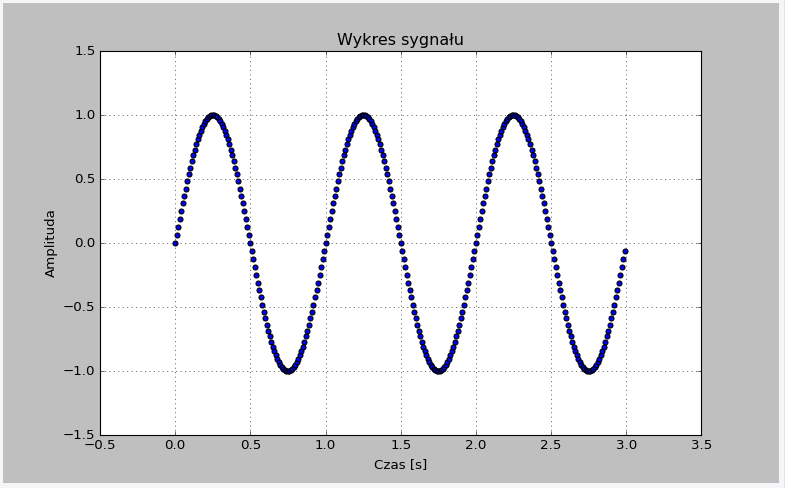
\includegraphics[width=0.7\textwidth]{img/splot1.png}
                \caption{Wykres sygnału numer 1}
            \end{figure}
            \FloatBarrier
            \begin{table}[h!]
                \centering
                \begin{tabular}{|l|l|l|l|l|}
                    \hline
                    Amplitiuda & Czas początkowy & \shortstack{Czas trwania \\ sygnału} & \shortstack{Okres \\ podstawowy} & \shortstack{Częstotliwość\\ próbkowania}   \\ \hline
                    2 & 1s & 3s & 1 & 100           \\ \hline
                \end{tabular}
                \caption{Parametry wejściowe dla sygnału nr 2}
            \end{table}
            \begin{figure}[h!]
                \centering
                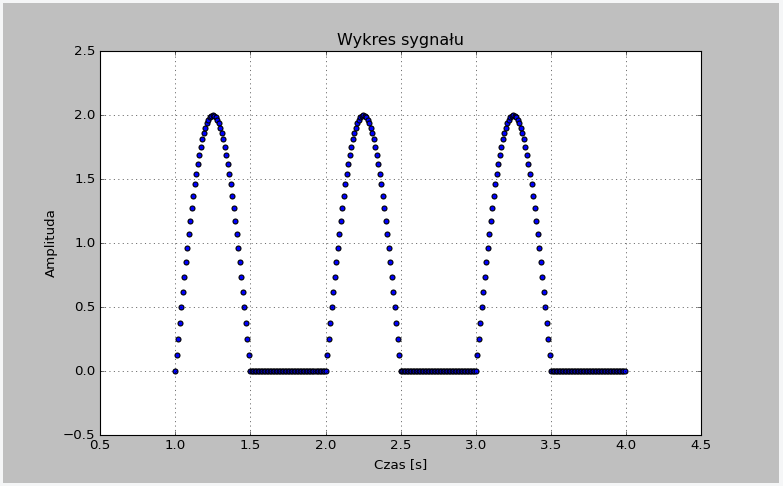
\includegraphics[width=0.7\textwidth]{img/splot4.png}
                \caption{Wykres sygnału numer 2}
            \end{figure}

            \begin{figure}[h!]
                \centering
                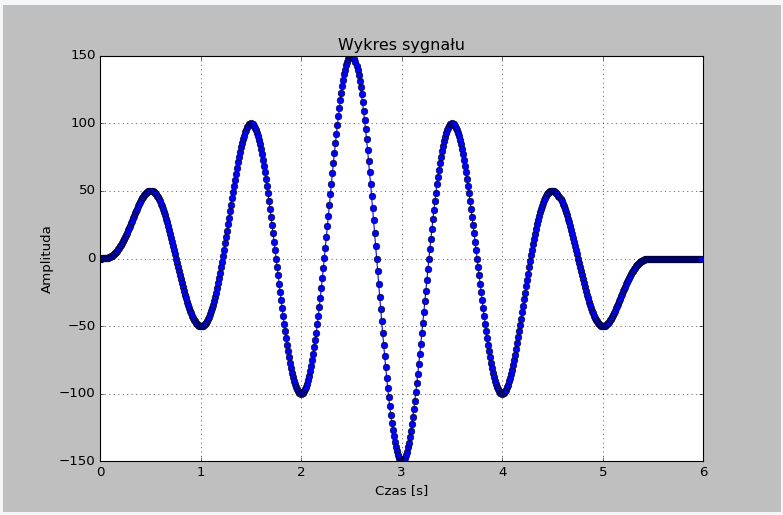
\includegraphics[width=0.7\textwidth]{img/splot5.png}
                \caption{Wykres sygnału po operacji splotu}
            \end{figure}
            \FloatBarrier
        }

        \subsubsection{Splot sygnałów sinusoidalnego oraz trójkątnego} \label{eksperyment:splot3}{

            \begin{table}[h!]
                \centering
                \begin{tabular}{|l|l|l|l|l|}
                    \hline
                    Amplitiuda & Czas początkowy & \shortstack{Czas trwania \\ sygnału} & \shortstack{Okres \\ podstawowy} & \shortstack{Częstotliwość\\ próbkowania}   \\ \hline
                    1 & 0s & 3s & 1 & 100           \\ \hline
                \end{tabular}
                \caption{Parametry wejściowe dla sygnału nr 1}
            \end{table}
            \FloatBarrier
            \begin{figure}[h!]
                \centering
                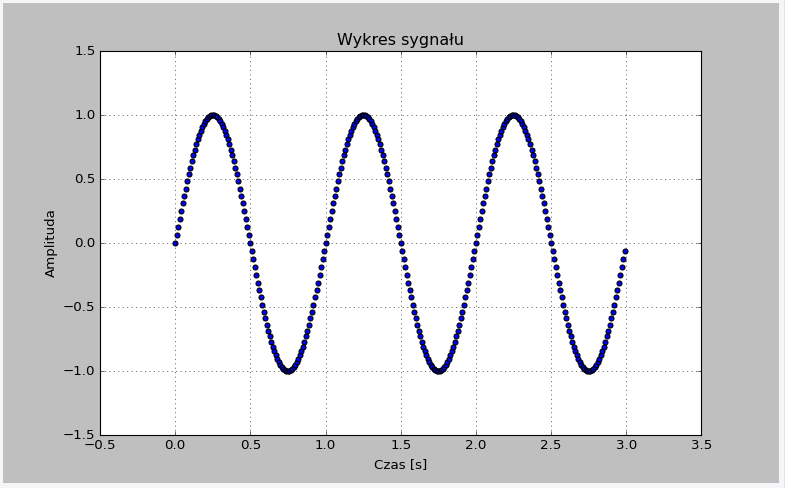
\includegraphics[width=0.7\textwidth]{img/splot1.png}
                \caption{Wykres sygnału numer 1}
            \end{figure}
            \FloatBarrier
            \begin{table}[h!]
                \centering
                \begin{tabular}{|l|l|l|l|l|l|}
                    \hline
                    Amplitiuda & \shortstack{Czas \\ początkowy} & \shortstack{Czas trwania \\ sygnału} & \shortstack{Okres \\ podstawowy} & \shortstack{Współczynnik\\ wypełnienia}  & \shortstack{Częstotliwość\\ próbkowania}   \\ \hline
                    2 & 0s & 3s & 0.5 & 0.5 & 70           \\ \hline
                \end{tabular}
                \caption{Parametry wejściowe dla sygnału nr 2}
            \end{table}
            \begin{figure}[h!]
                \centering
                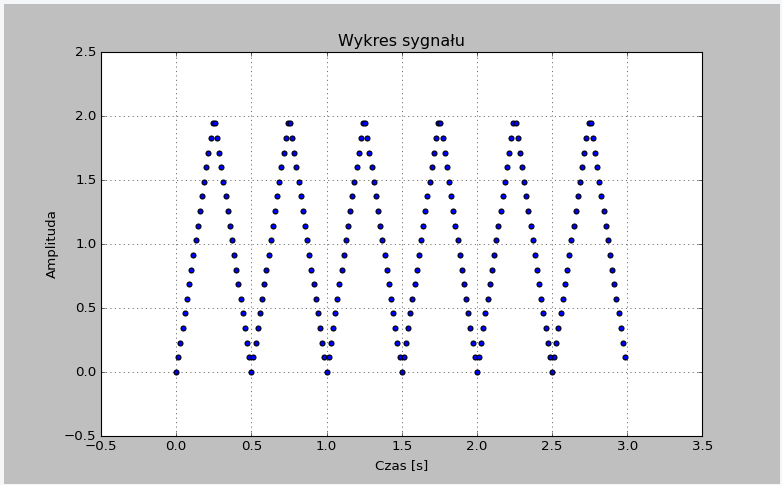
\includegraphics[width=0.7\textwidth]{img/splot6.png}
                \caption{Wykres sygnału numer 2}
            \end{figure}

            \begin{figure}[h!]
                \centering
                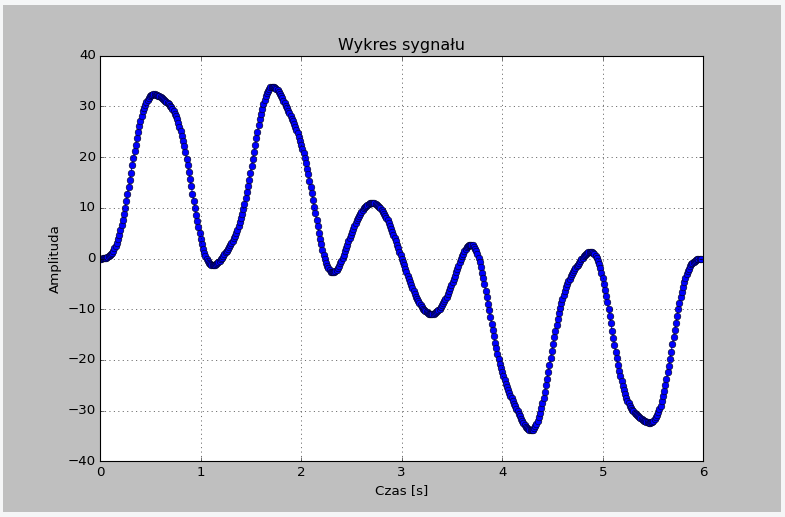
\includegraphics[width=0.7\textwidth]{img/splot7.png}
                \caption{Wykres sygnału po operacji splotu}
            \end{figure}
            \FloatBarrier
        }
        \subsubsection{Korelacja bezpośrednia sygnałów sinusoidalnych} \label{eksperyment:korelacja1}{

        \begin{table}[h!]
            \centering
            \begin{tabular}{|l|l|l|l|l|}
                \hline
                Amplitiuda & Czas początkowy & \shortstack{Czas trwania \\ sygnału} & \shortstack{Okres \\ podstawowy} & \shortstack{Częstotliwość\\ próbkowania}   \\ \hline
                1 & 0s & 3s & 1 & 100           \\ \hline
            \end{tabular}
            \caption{Parametry wejściowe dla sygnału nr 1}
        \end{table}
        \begin{figure}[h!]
            \centering
            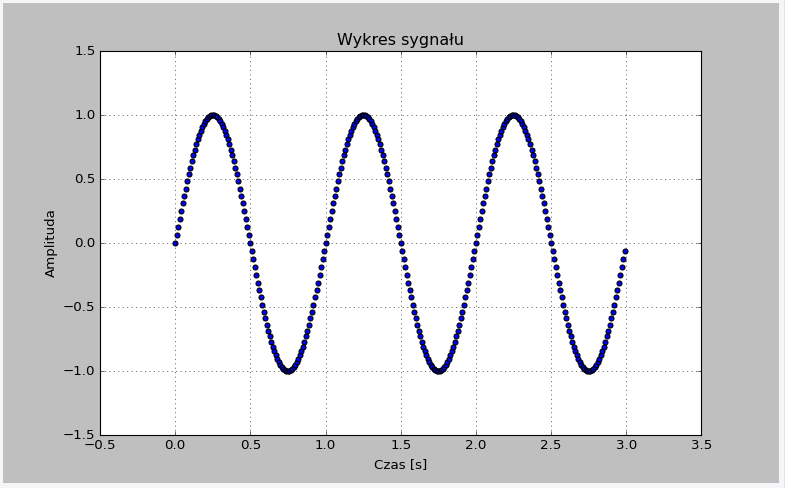
\includegraphics[width=0.7\textwidth]{img/splot1.png}
            \caption{Wykres sygnału numer 1}
        \end{figure}
        \FloatBarrier
        \begin{table}[h!]
            \centering
            \begin{tabular}{|l|l|l|l|l|}
                \hline
                Amplitiuda & Czas początkowy & \shortstack{Czas trwania \\ sygnału} & \shortstack{Okres \\ podstawowy} & \shortstack{Częstotliwość\\ próbkowania}   \\ \hline
                1 & 2s & 3s & 1 & 100           \\ \hline
            \end{tabular}
            \caption{Parametry wejściowe dla sygnału nr 2}
        \end{table}
        \begin{figure}[h!]
            \centering
            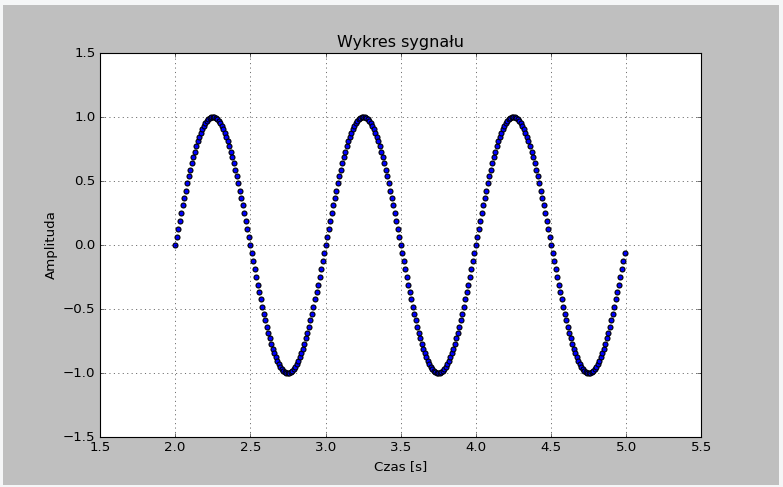
\includegraphics[width=0.7\textwidth]{img/splot2.png}
            \caption{Wykres sygnału numer 2}
        \end{figure}

        \begin{figure}[h!]
            \centering
            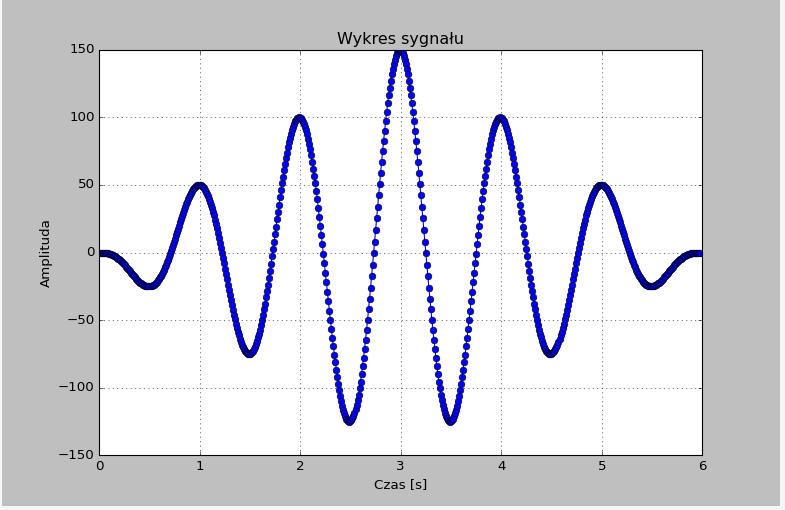
\includegraphics[width=0.7\textwidth]{img/kor_bez_1.png}
            \caption{Wykres sygnału po operacji korelacji}
        \end{figure}
        \FloatBarrier
    }
    \FloatBarrier
\subsubsection{Korelacja bezpośrednia sinsoidalnego oraz sinusoidalnego wyprostowanego
    jednopołówkowo} \label{eksperyment:korelacja2}{

    \begin{table}[h!]
        \centering
        \begin{tabular}{|l|l|l|l|l|}
            \hline
            Amplitiuda & Czas początkowy & \shortstack{Czas trwania \\ sygnału} & \shortstack{Okres \\ podstawowy} & \shortstack{Częstotliwość\\ próbkowania}   \\ \hline
            1 & 0s & 3s & 1 & 100           \\ \hline
        \end{tabular}
        \caption{Parametry wejściowe dla sygnału nr 1}
    \end{table}
    \begin{figure}[h!]
        \centering
        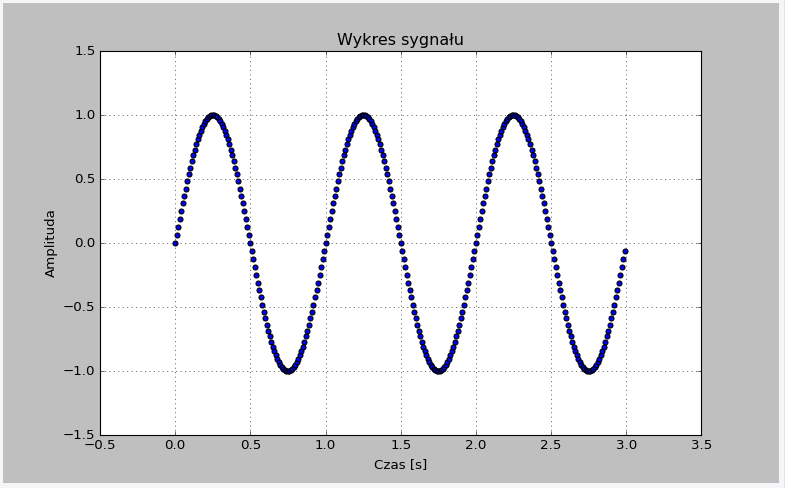
\includegraphics[width=0.7\textwidth]{img/splot1.png}
        \caption{Wykres sygnału numer 1}
    \end{figure}
    \FloatBarrier
    \begin{table}[h!]
        \centering
        \begin{tabular}{|l|l|l|l|l|}
            \hline
            Amplitiuda & Czas początkowy & \shortstack{Czas trwania \\ sygnału} & \shortstack{Okres \\ podstawowy} & \shortstack{Częstotliwość\\ próbkowania}   \\ \hline
            2 & 1s & 3s & 1 & 100           \\ \hline
        \end{tabular}
        \caption{Parametry wejściowe dla sygnału nr 2}
    \end{table}
    \begin{figure}[h!]
        \centering
        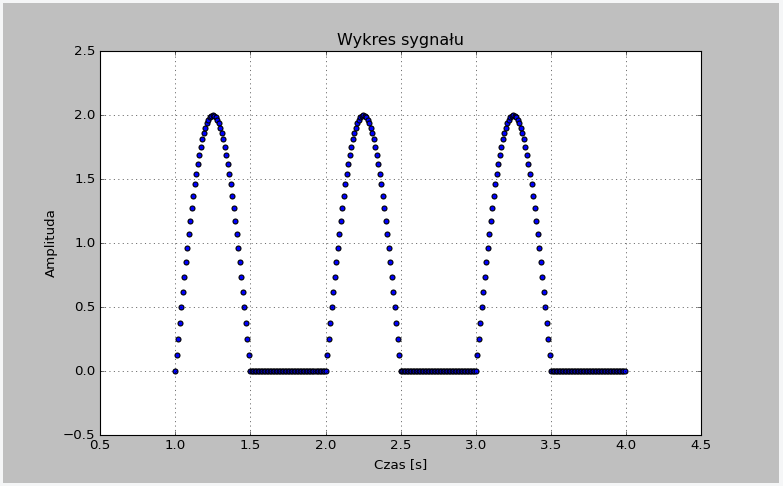
\includegraphics[width=0.7\textwidth]{img/splot4.png}
        \caption{Wykres sygnału numer 2}
    \end{figure}

    \begin{figure}[h!]
        \centering
        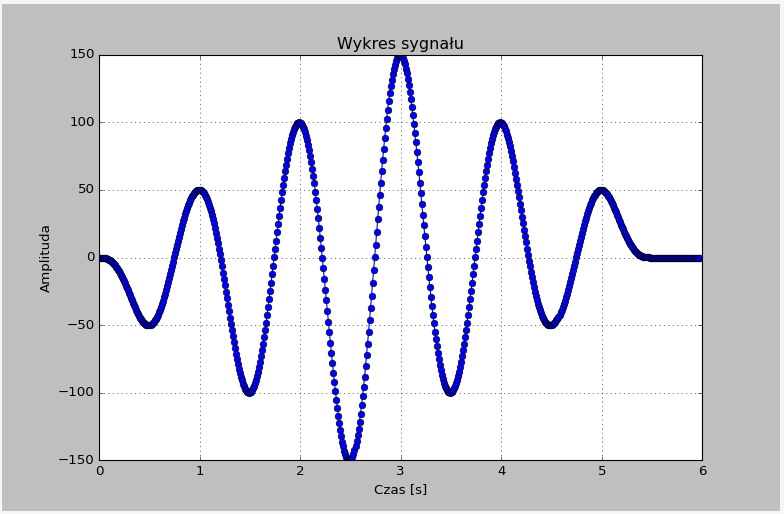
\includegraphics[width=0.7\textwidth]{img/kor_bez_2.png}
        \caption{Wykres sygnału po operacji korelacji}
    \end{figure}
}

\subsubsection{Korelacja bezpośrednia sygnałów sinusoidalnego oraz trójkątnego} \label{eksperyment:korelacja3}{

    \begin{table}[h!]
        \centering
        \begin{tabular}{|l|l|l|l|l|}
            \hline
            Amplitiuda & Czas początkowy & \shortstack{Czas trwania \\ sygnału} & \shortstack{Okres \\ podstawowy} & \shortstack{Częstotliwość\\ próbkowania}   \\ \hline
            1 & 0s & 3s & 1 & 100           \\ \hline
        \end{tabular}
        \caption{Parametry wejściowe dla sygnału nr 1}
    \end{table}
    \FloatBarrier
    \begin{figure}[h!]
        \centering
        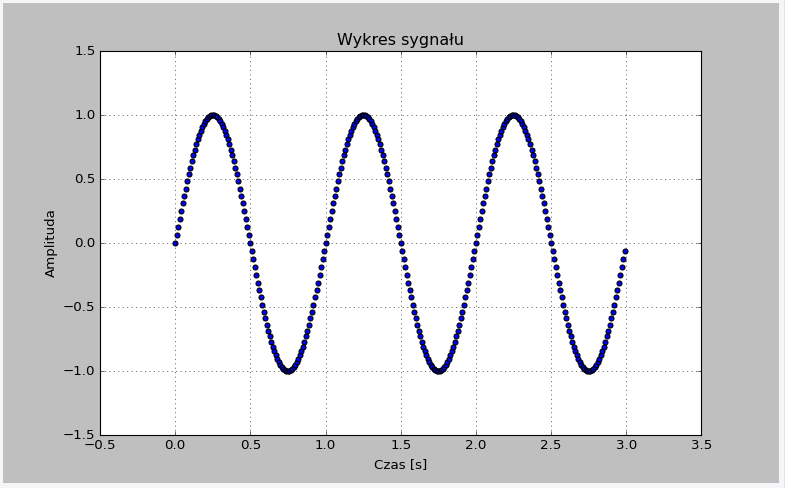
\includegraphics[width=0.7\textwidth]{img/splot1.png}
        \caption{Wykres sygnału numer 1}
    \end{figure}
    \FloatBarrier
    \begin{table}[h!]
        \centering
        \begin{tabular}{|l|l|l|l|l|l|}
            \hline
            Amplitiuda & \shortstack{Czas \\ początkowy} & \shortstack{Czas trwania \\ sygnału} & \shortstack{Okres \\ podstawowy} & \shortstack{Współczynnik\\ wypełnienia}  & \shortstack{Częstotliwość\\ próbkowania}   \\ \hline
            2 & 0s & 3s & 0.5 & 0.5 & 70           \\ \hline
        \end{tabular}
        \caption{Parametry wejściowe dla sygnału nr 2}
    \end{table}
    \begin{figure}[h!]
        \centering
        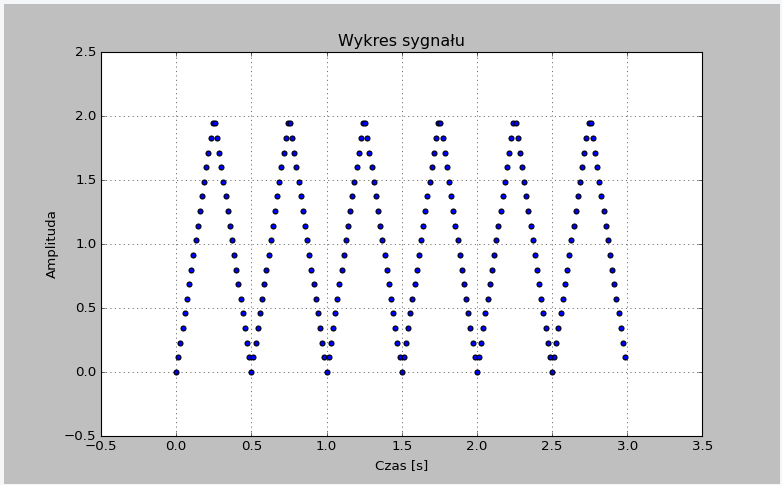
\includegraphics[width=0.7\textwidth]{img/splot6.png}
        \caption{Wykres sygnału numer 2}
    \end{figure}

    \begin{figure}[h!]
        \centering
        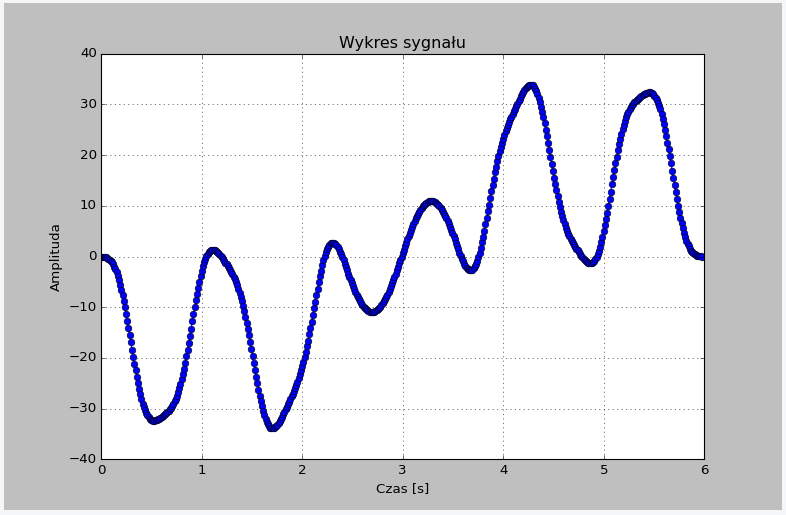
\includegraphics[width=0.7\textwidth]{img/kor_bez_3.png}
        \caption{Wykres sygnału po operacji korelacji}
    \end{figure}
    \FloatBarrier
    
}
    \subsubsection{Korelacja z użyciem splotu sygnałów sinusoidalnych} \label{eksperyment:korelacja4}{

    \begin{table}[h!]
        \centering
        \begin{tabular}{|l|l|l|l|l|}
            \hline
            Amplitiuda & Czas początkowy & \shortstack{Czas trwania \\ sygnału} & \shortstack{Okres \\ podstawowy} & \shortstack{Częstotliwość\\ próbkowania}   \\ \hline
            1 & 0s & 3s & 1 & 100           \\ \hline
        \end{tabular}
        \caption{Parametry wejściowe dla sygnału nr 1}
    \end{table}
    \begin{figure}[h!]
        \centering
        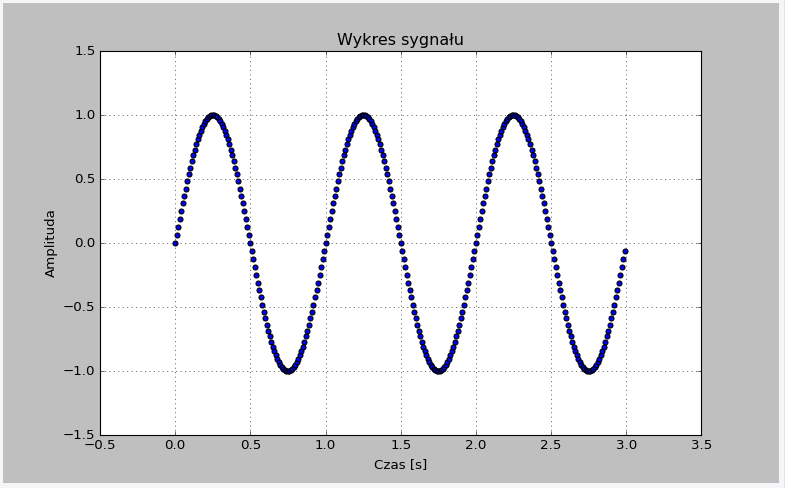
\includegraphics[width=0.7\textwidth]{img/splot1.png}
        \caption{Wykres sygnału numer 1}
    \end{figure}

    \begin{table}[h!]
        \centering
        \begin{tabular}{|l|l|l|l|l|}
            \hline
            Amplitiuda & Czas początkowy & \shortstack{Czas trwania \\ sygnału} & \shortstack{Okres \\ podstawowy} & \shortstack{Częstotliwość\\ próbkowania}   \\ \hline
            1 & 2s & 3s & 1 & 100           \\ \hline
        \end{tabular}
        \caption{Parametry wejściowe dla sygnału nr 2}
    \end{table}
    \begin{figure}[h!]
        \centering
        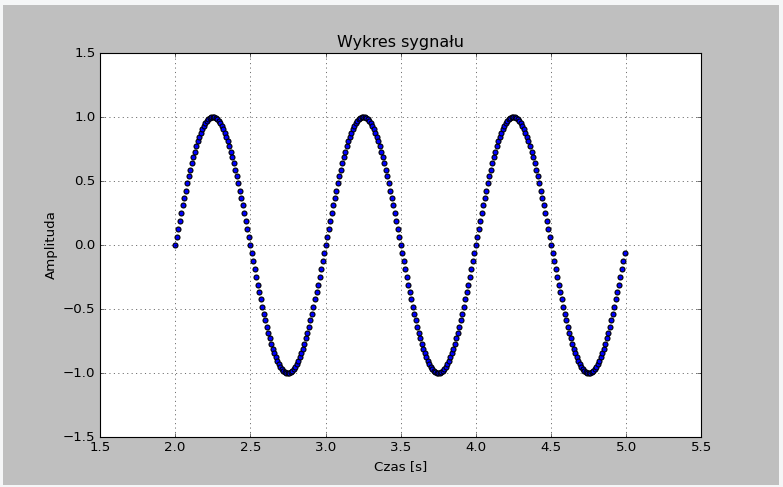
\includegraphics[width=0.7\textwidth]{img/splot2.png}
        \caption{Wykres sygnału numer 2}
    \end{figure}

    \begin{figure}[h!]
        \centering
        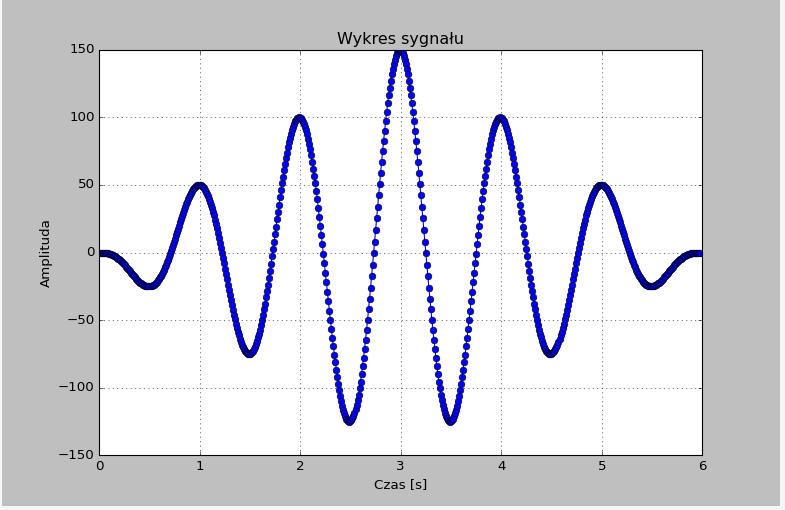
\includegraphics[width=0.7\textwidth]{img/kor_bez_1.png}
        \caption{Wykres sygnału po operacji korelacji}
    \end{figure}
    }
    \FloatBarrier
    \subsubsection{Korelacja z użyciem splotu sinsoidalnego oraz sinusoidalnego wyprostowanego
    jednopołówkowo} \label{eksperyment:korelacja5}{

    \begin{table}[h!]
    \centering
    \begin{tabular}{|l|l|l|l|l|}
        \hline
        Amplitiuda & Czas początkowy & \shortstack{Czas trwania \\ sygnału} & \shortstack{Okres \\ podstawowy} & \shortstack{Częstotliwość\\ próbkowania}   \\ \hline
        1 & 0s & 3s & 1 & 100           \\ \hline
    \end{tabular}
    \caption{Parametry wejściowe dla sygnału nr 1}
    \end{table}
    \begin{figure}[h!]
    \centering
    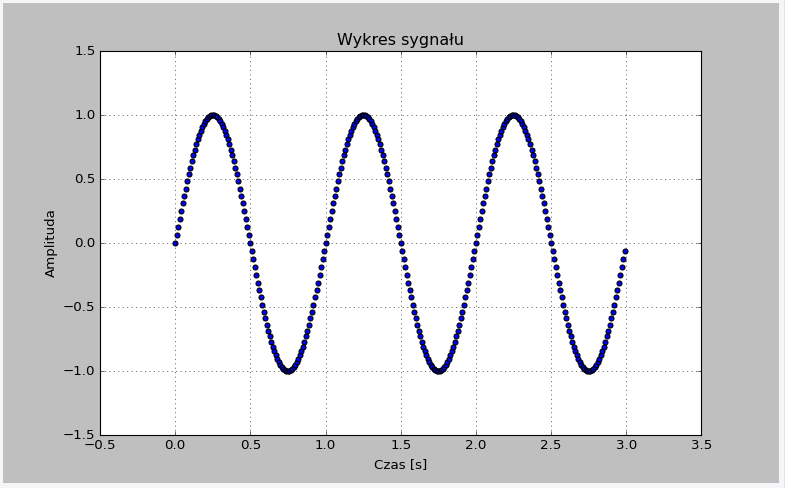
\includegraphics[width=0.7\textwidth]{img/splot1.png}
    \caption{Wykres sygnału numer 1}
    \end{figure}
    \FloatBarrier
    \begin{table}[h!]
    \centering
    \begin{tabular}{|l|l|l|l|l|}
        \hline
        Amplitiuda & Czas początkowy & \shortstack{Czas trwania \\ sygnału} & \shortstack{Okres \\ podstawowy} & \shortstack{Częstotliwość\\ próbkowania}   \\ \hline
        2 & 1s & 3s & 1 & 100           \\ \hline
    \end{tabular}
    \caption{Parametry wejściowe dla sygnału nr 2}
    \end{table}
    \begin{figure}[h!]
    \centering
    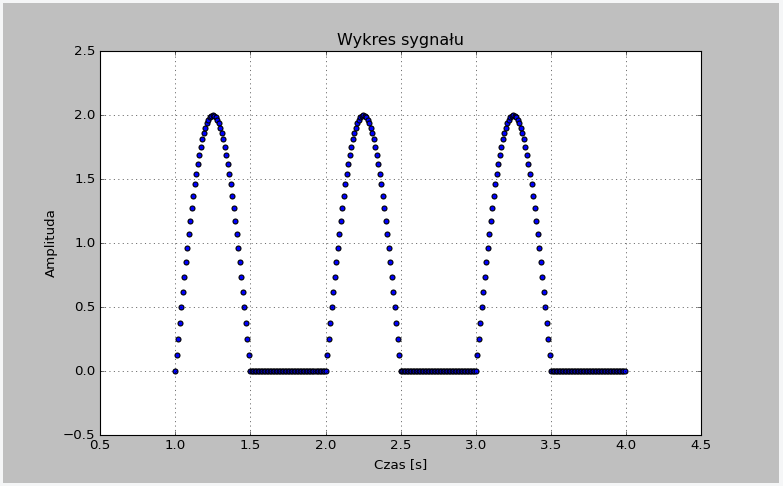
\includegraphics[width=0.7\textwidth]{img/splot4.png}
    \caption{Wykres sygnału numer 2}
    \end{figure}

    \begin{figure}[h!]
    \centering
    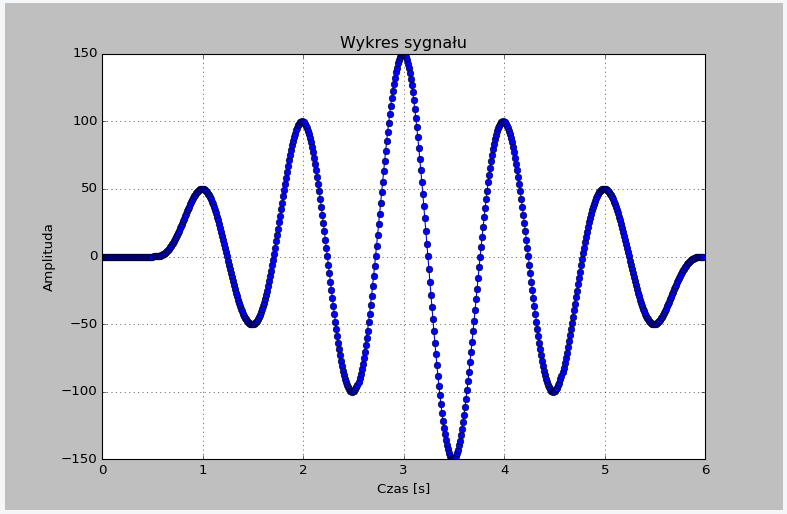
\includegraphics[width=0.7\textwidth]{img/kor_2.png}
    \caption{Wykres sygnału po operacji korelacji}
    \end{figure}
    \FloatBarrier
    }

    \subsubsection{Korelacja z użyciem splotu sygnałów sinusoidalnego oraz trójkątnego} \label{eksperyment:korelacja6}{

    \begin{table}[h!]
    \centering
    \begin{tabular}{|l|l|l|l|l|}
        \hline
        Amplitiuda & Czas początkowy & \shortstack{Czas trwania \\ sygnału} & \shortstack{Okres \\ podstawowy} & \shortstack{Częstotliwość\\ próbkowania}   \\ \hline
        1 & 0s & 3s & 1 & 100           \\ \hline
    \end{tabular}
    \caption{Parametry wejściowe dla sygnału nr 1}
    \end{table}
    \FloatBarrier
    \begin{figure}[h!]
    \centering
    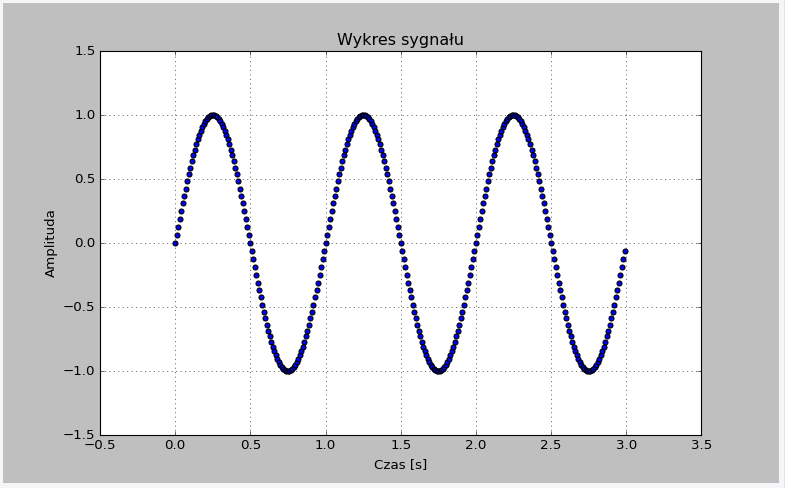
\includegraphics[width=0.7\textwidth]{img/splot1.png}
    \caption{Wykres sygnału numer 1}
    \end{figure}
    \FloatBarrier
    \begin{table}[h!]
    \centering
    \begin{tabular}{|l|l|l|l|l|l|}
        \hline
        Amplitiuda & \shortstack{Czas \\ początkowy} & \shortstack{Czas trwania \\ sygnału} & \shortstack{Okres \\ podstawowy} & \shortstack{Współczynnik\\ wypełnienia}  & \shortstack{Częstotliwość\\ próbkowania}   \\ \hline
        2 & 0s & 3s & 0.5 & 0.5 & 70           \\ \hline
    \end{tabular}
    \caption{Parametry wejściowe dla sygnału nr 2}
    \end{table}
    \begin{figure}[h!]
    \centering
    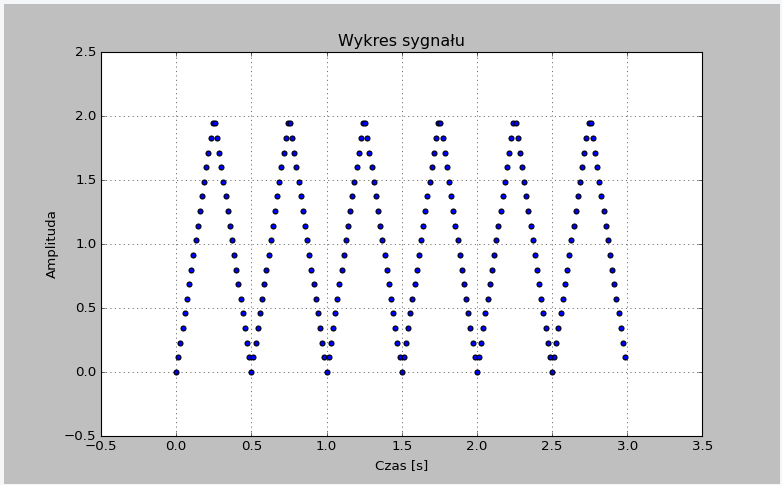
\includegraphics[width=0.7\textwidth]{img/splot6.png}
    \caption{Wykres sygnału numer 2}
    \end{figure}

    \begin{figure}[h!]
    \centering
    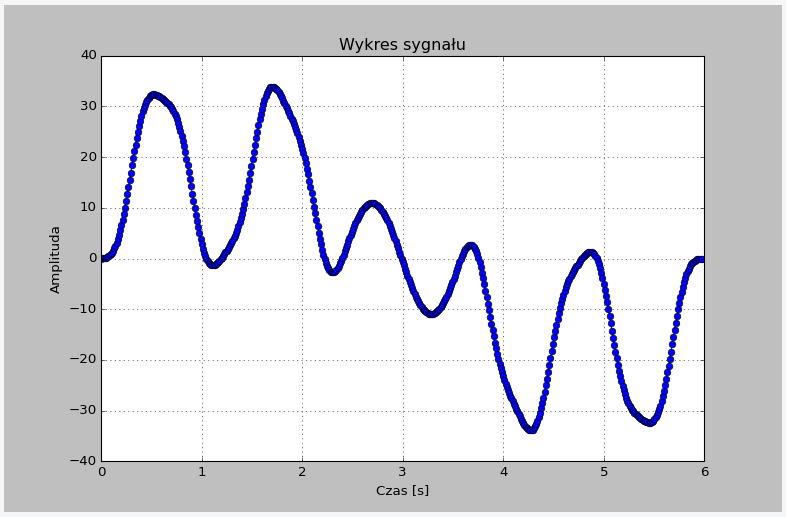
\includegraphics[width=0.7\textwidth]{img/kor_3.png}
    \caption{Wykres sygnału po operacji korelacji}
    \end{figure}
    \FloatBarrier
    }
}

    \subsection{Filtracja sygnałów dyskretnych} {
        \subsubsection{Eksperyment 1} {
            \begin{table}[h!]
            \centering
            \begin{tabular}{|l|l|l|l|l|l|}
            \hline
            Typ filtra & Rząd filtra & Częstotliwość odcięcia & Typ okna  \\\hline
            Dolnoprzepustowy & 51 & 5 & rectangular     \\\hline
            \end{tabular}
            \caption{Parametry filtra}
            \end{table}
            \begin{figure}[h!]
                \centering
                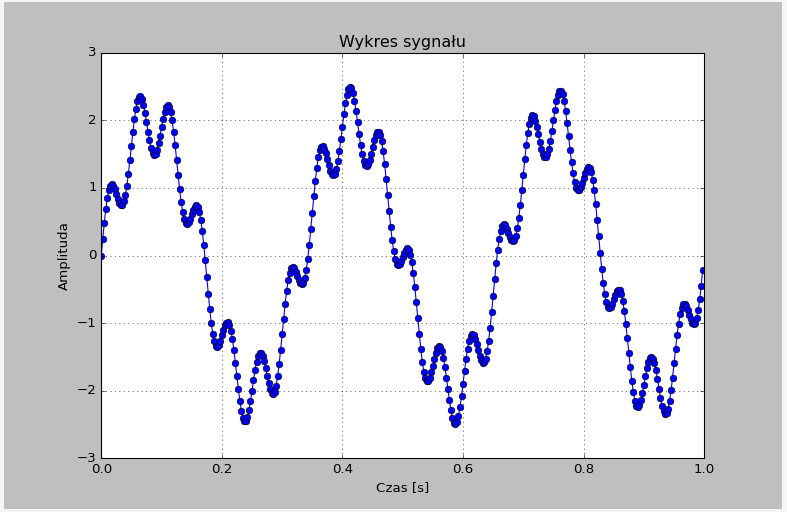
\includegraphics[width=0.7\textwidth]{img/sig.png}
                \caption{Wykres sygnału przed filtracją}
            \end{figure}
            \begin{figure}[h!]
                \centering
                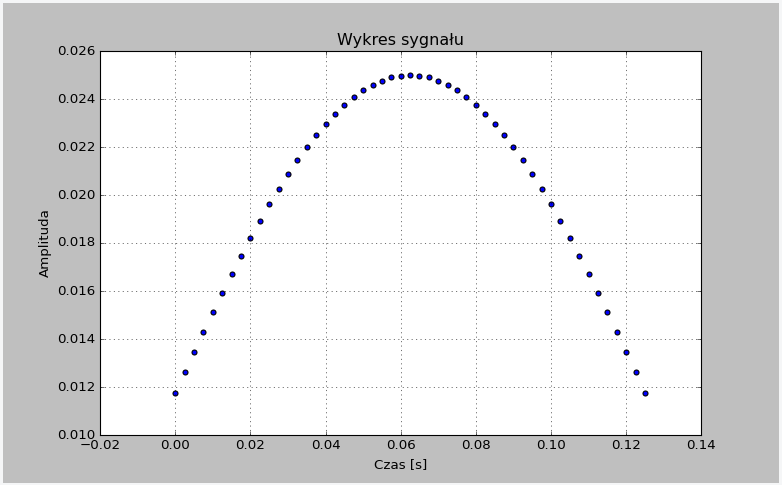
\includegraphics[width=0.7\textwidth]{img/fil1.png}
                \caption{Wykres filtra}
            \end{figure}

            \begin{figure}[h!]
                \centering
                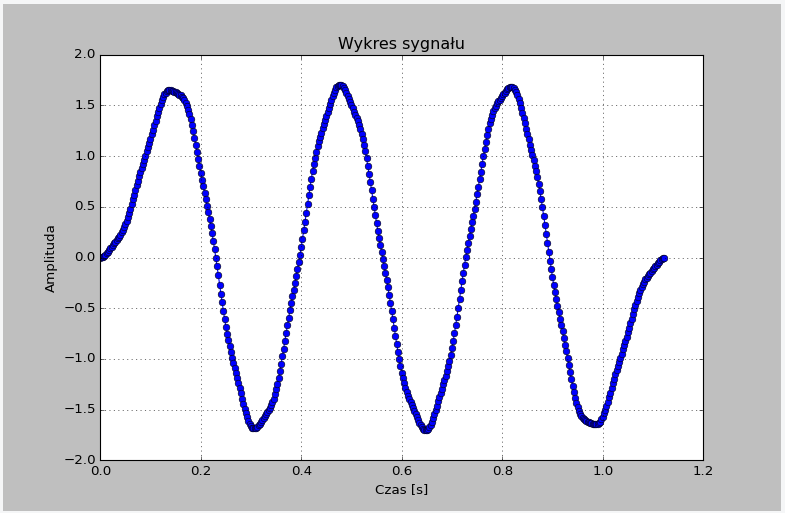
\includegraphics[width=0.7\textwidth]{img/fil2.png}
                \caption{Wykres sygnału po filtracji}
            \end{figure}
            \FloatBarrier
        }
        \newpage

        \subsubsection{Eksperyment 2} {
            \begin{table}[h!]
            \centering
            \begin{tabular}{|l|l|l|l|l|l|}
            \hline
            Typ filtra & Rząd filtra & Częstotliwość odciecia & Typ okna  \\\hline
            Dolnoprzepustowy & 51 & 5 & hamming     \\\hline
            \end{tabular}
            \caption{Parametry filtra}
            \end{table}
            \begin{figure}[h!]
                \centering
                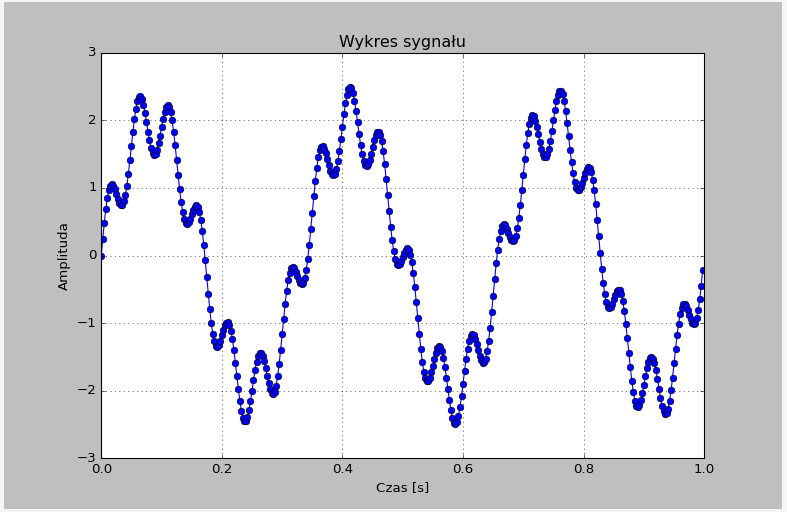
\includegraphics[width=0.7\textwidth]{img/sig.png}
                \caption{Wykres sygnału przed filtracją}
            \end{figure}
            \begin{figure}[h!]
                \centering
                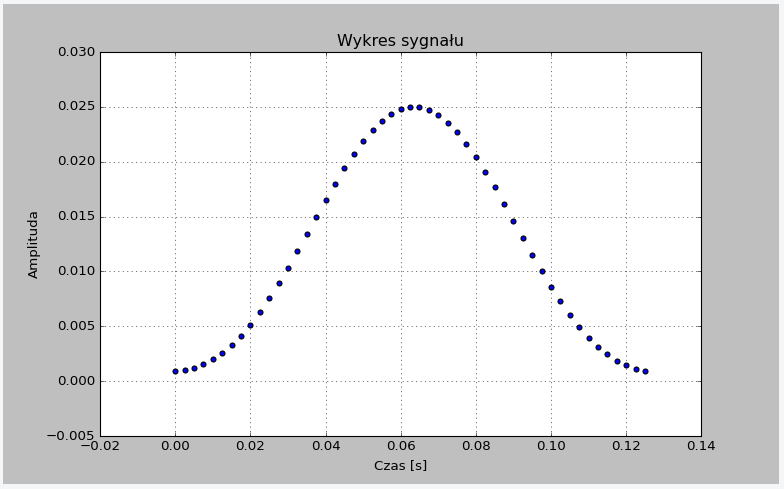
\includegraphics[width=0.7\textwidth]{img/fil3.png}
                \caption{Wykres filtra}
            \end{figure}

            \begin{figure}[h!]
                \centering
                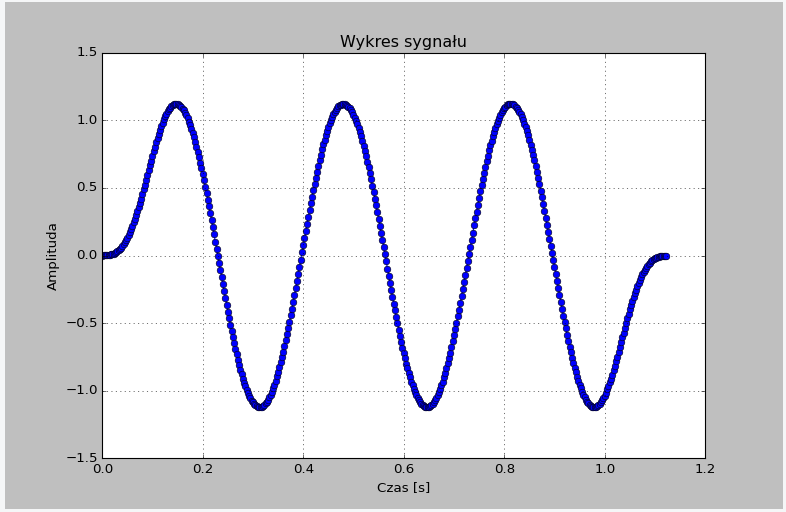
\includegraphics[width=0.7\textwidth]{img/fil4.png}
                \caption{Wykres sygnału po filtracji}
            \end{figure}
            \FloatBarrier
        }
        \newpage

        \subsubsection{Eksperyment 3} {
            \begin{table}[h!]
            \centering
            \begin{tabular}{|l|l|l|l|l|l|}
            \hline
            Typ filtra & Rząd filtra & Częstotliwość odciecia & Typ okna  \\\hline
            Dolnoprzepustowy & 51 & 5 & hanning     \\\hline
            \end{tabular}
            \caption{Parametry filtra}
            \end{table}
            \begin{figure}[h!]
                \centering
                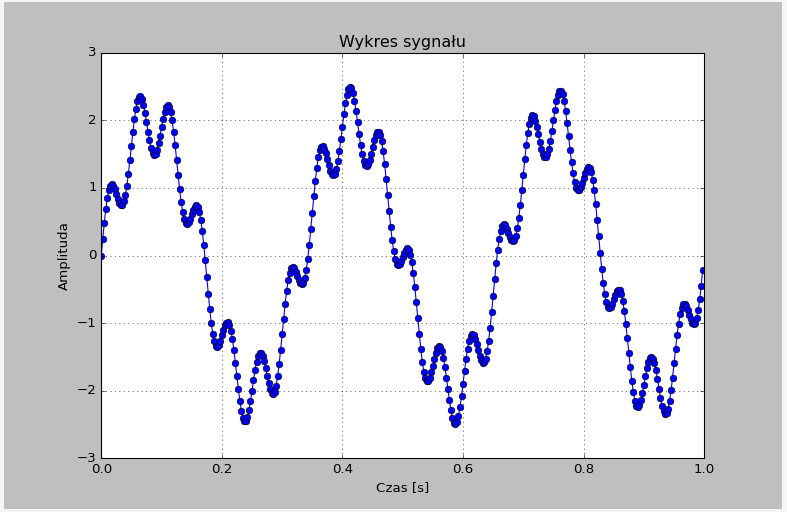
\includegraphics[width=0.7\textwidth]{img/sig.png}
                \caption{Wykres sygnału przed filtracją}
            \end{figure}
            \begin{figure}[h!]
                \centering
                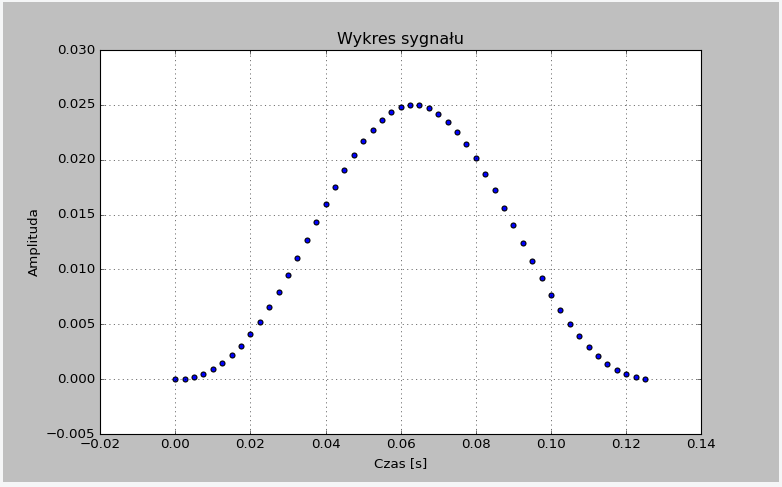
\includegraphics[width=0.7\textwidth]{img/fil5.png}
                \caption{Wykres filtra}
            \end{figure}

            \begin{figure}[h!]
                \centering
                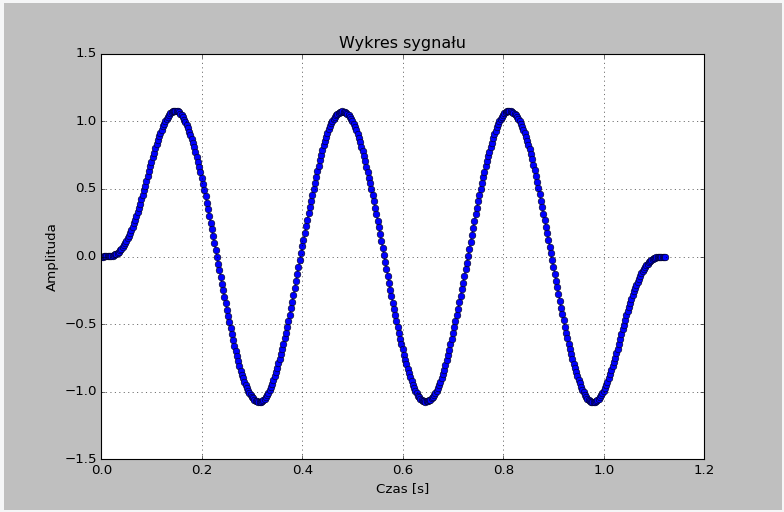
\includegraphics[width=0.7\textwidth]{img/fil6.png}
                \caption{Wykres sygnału po filtracji}
            \end{figure}
            \FloatBarrier
        }
        \newpage

        \subsubsection{Eksperyment 4} {
            \begin{table}[h!]
            \centering
            \begin{tabular}{|l|l|l|l|l|l|}
            \hline
            Typ filtra & Rząd filtra & Częstotliwość odciecia & Typ okna  \\\hline
            Dolnoprzepustowy & 51 & 5 & blackman     \\\hline
            \end{tabular}
            \caption{Parametry filtra}
            \end{table}
            \begin{figure}[h!]
                \centering
                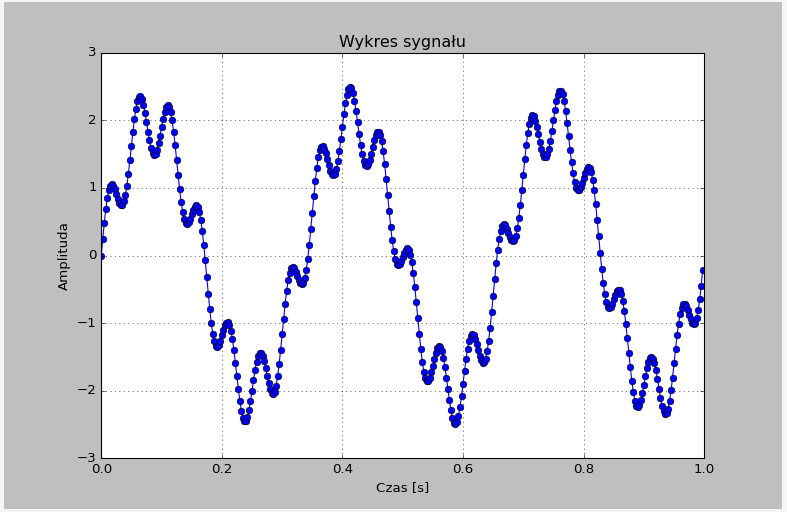
\includegraphics[width=0.7\textwidth]{img/sig.png}
                \caption{Wykres sygnału przed filtracją}
            \end{figure}
            \begin{figure}[h!]
                \centering
                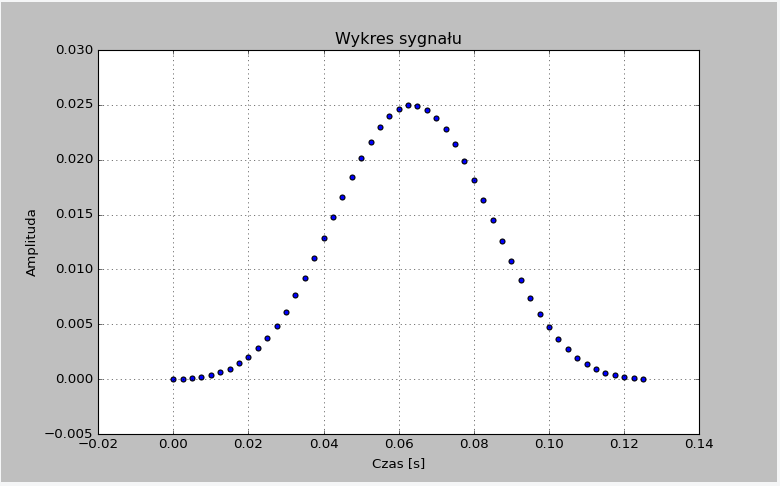
\includegraphics[width=0.7\textwidth]{img/fil7.png}
                \caption{Wykres filtra}
            \end{figure}

            \begin{figure}[h!]
                \centering
                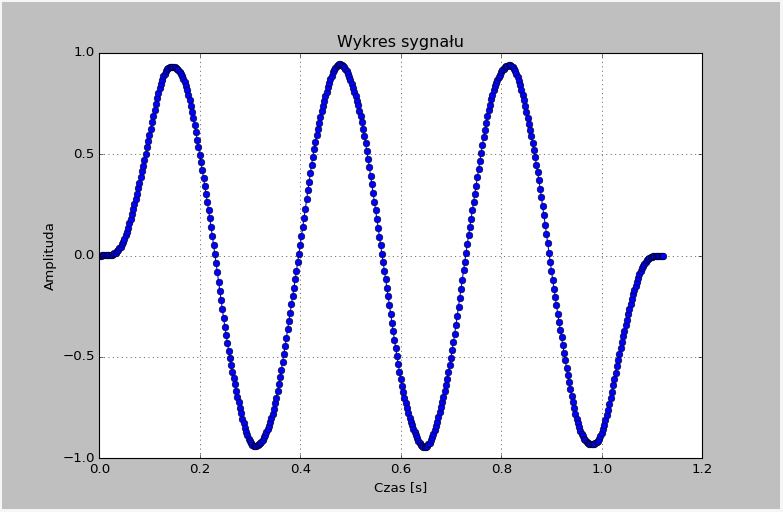
\includegraphics[width=0.7\textwidth]{img/fil8.png}
                \caption{Wykres sygnału po filtracji}
            \end{figure}
            \FloatBarrier
        }
        \newpage

        \subsubsection{Eksperyment 5} {
            \begin{table}[h!]
            \centering
            \begin{tabular}{|l|l|l|l|l|l|}
            \hline
            Typ filtra & Rząd filtra & Częstotliwość odciecia & Typ okna  \\\hline
            Dolnoprzepustowy & 41 & 5 & hamming     \\\hline
            \end{tabular}
            \caption{Parametry filtra}
            \end{table}
            \begin{figure}[h!]
                \centering
                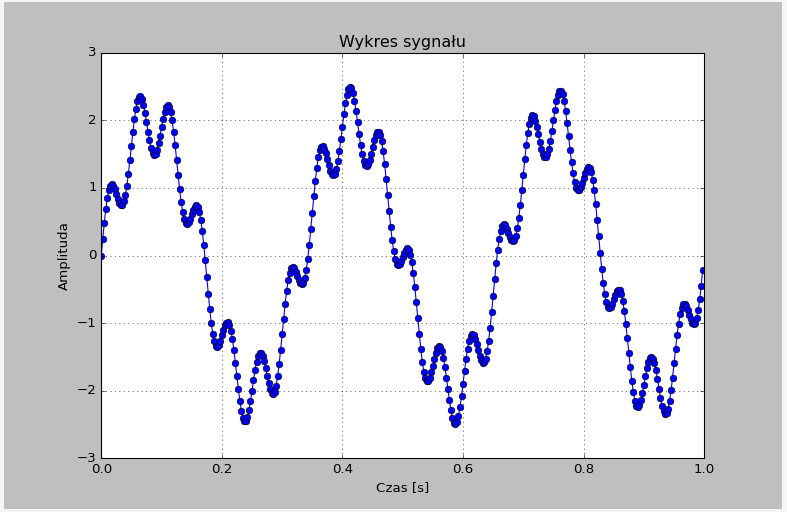
\includegraphics[width=0.7\textwidth]{img/sig.png}
                \caption{Wykres sygnału przed filtracją}
            \end{figure}
            \begin{figure}[h!]
                \centering
                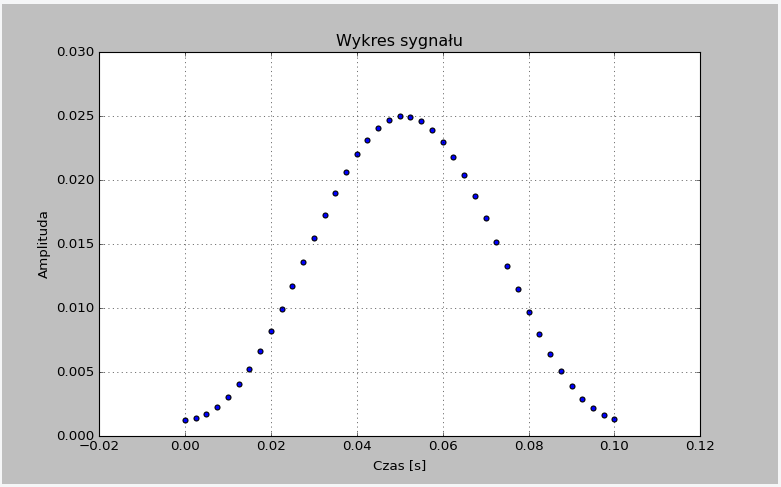
\includegraphics[width=0.7\textwidth]{img/fil9.png}
                \caption{Wykres filtra}
            \end{figure}

            \begin{figure}[h!]
                \centering
                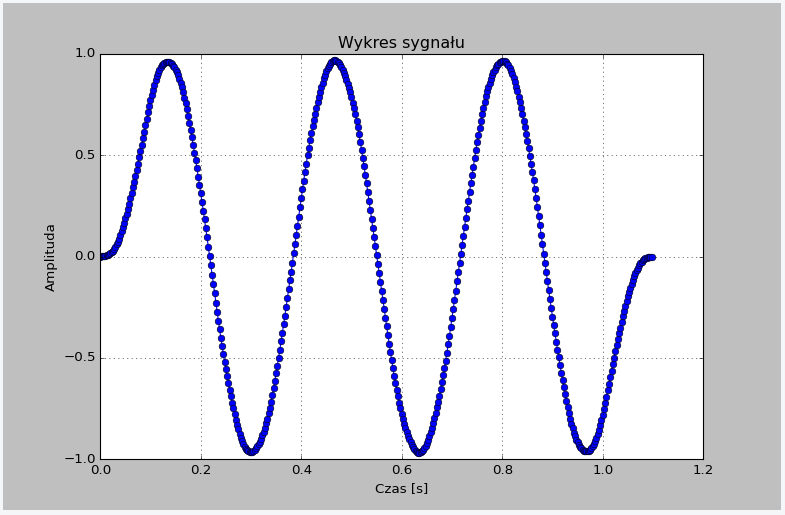
\includegraphics[width=0.7\textwidth]{img/fil10.png}
                \caption{Wykres sygnału po filtracji}
            \end{figure}
            \FloatBarrier
        }
        \newpage

        \subsubsection{Eksperyment 6} {
            \begin{table}[h!]
            \centering
            \begin{tabular}{|l|l|l|l|l|l|}
            \hline
            Typ filtra & Rząd filtra & Częstotliwość odciecia & Typ okna  \\\hline
            Dolnoprzepustowy & 31 & 5 & hamming     \\\hline
            \end{tabular}
            \caption{Parametry filtra}
            \end{table}
            \begin{figure}[h!]
                \centering
                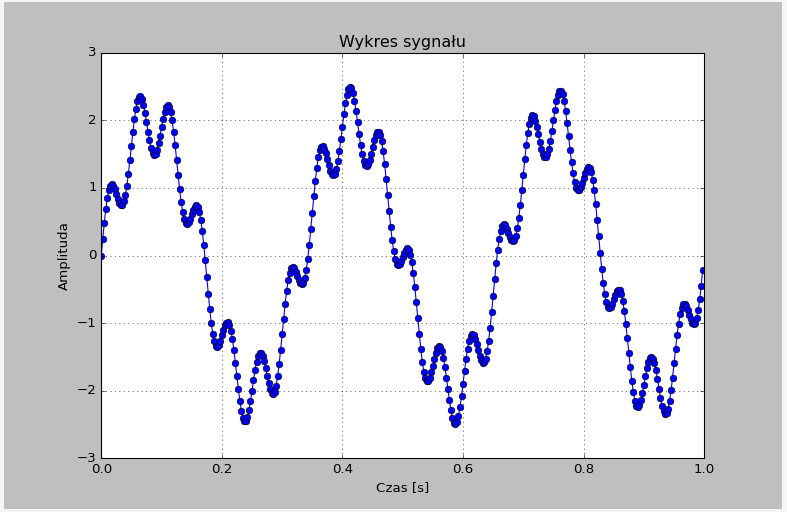
\includegraphics[width=0.7\textwidth]{img/sig.png}
                \caption{Wykres sygnału przed filtracją}
            \end{figure}
            \begin{figure}[h!]
                \centering
                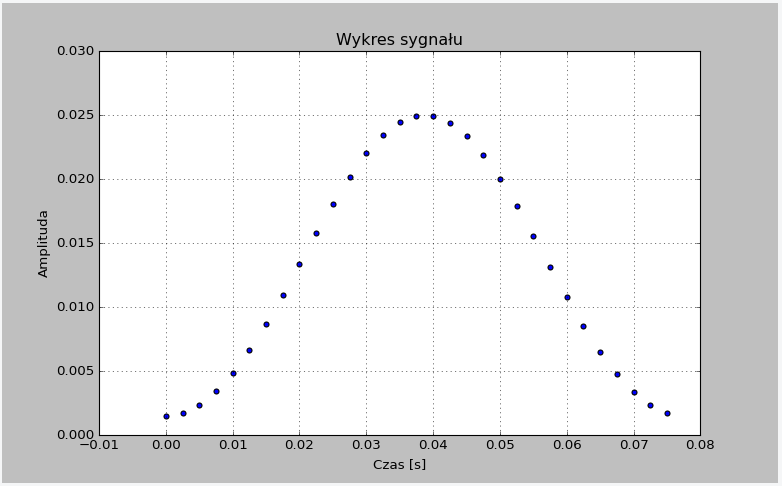
\includegraphics[width=0.7\textwidth]{img/fil11.png}
                \caption{Wykres filtra}
            \end{figure}

            \begin{figure}[h!]
                \centering
                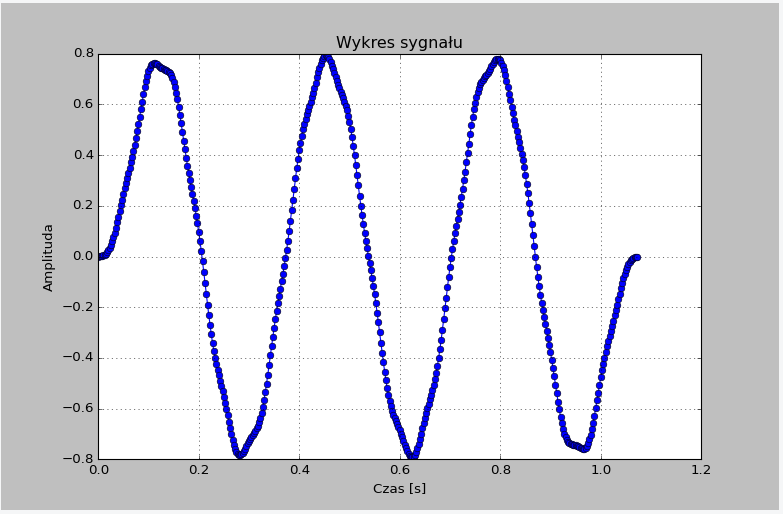
\includegraphics[width=0.7\textwidth]{img/fil12.png}
                \caption{Wykres sygnału po filtracji}
            \end{figure}
            \FloatBarrier
        }
        \newpage

        \subsubsection{Eksperyment 7} {
            \begin{table}[h!]
            \centering
            \begin{tabular}{|l|l|l|l|l|l|}
            \hline
            Typ filtra & Rząd filtra & Częstotliwość odciecia & Typ okna  \\\hline
            Dolnoprzepustowy & 21 & 5 & hamming     \\\hline
            \end{tabular}
            \caption{Parametry filtra}
            \end{table}
            \begin{figure}[h!]
                \centering
                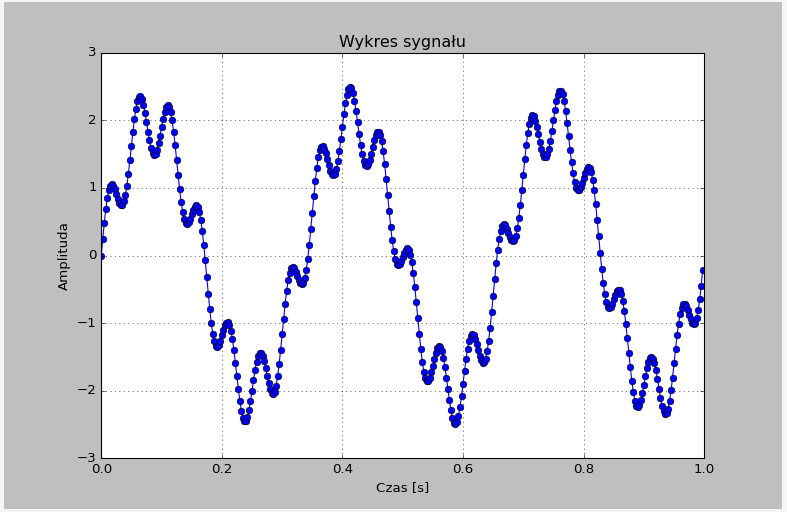
\includegraphics[width=0.7\textwidth]{img/sig.png}
                \caption{Wykres sygnału przed filtracją}
            \end{figure}
            \begin{figure}[h!]
                \centering
                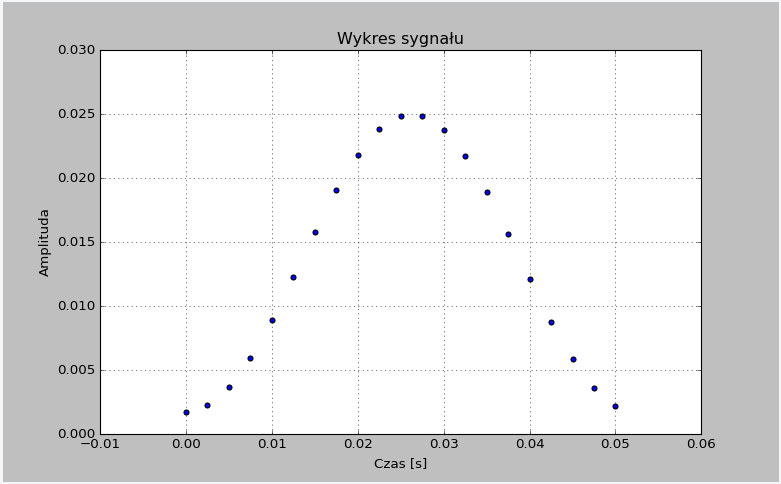
\includegraphics[width=0.7\textwidth]{img/fil13.png}
                \caption{Wykres filtra}
            \end{figure}

            \begin{figure}[h!]
                \centering
                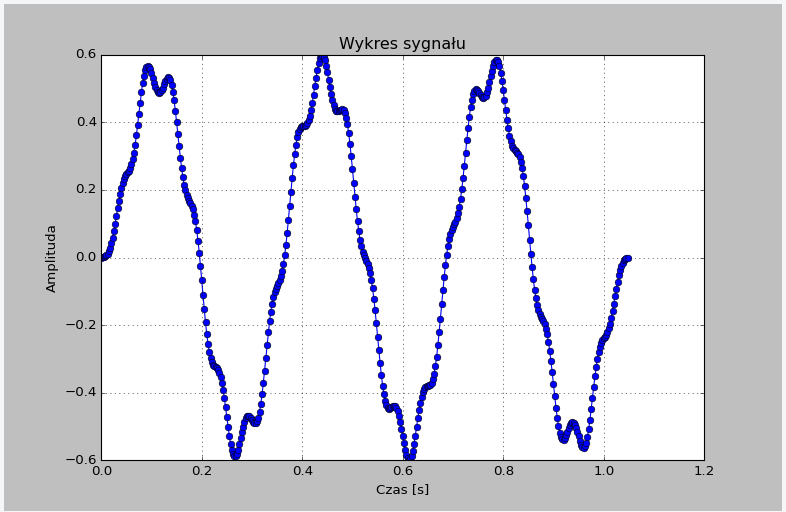
\includegraphics[width=0.7\textwidth]{img/fil14.png}
                \caption{Wykres sygnału po filtracji}
            \end{figure}
            \FloatBarrier
        }
        \newpage

        \subsubsection{Eksperyment 8} {
            \begin{table}[h!]
            \centering
            \begin{tabular}{|l|l|l|l|l|l|}
            \hline
            Typ filtra & Rząd filtra & Częstotliwość odciecia & Typ okna  \\\hline
            Dolnoprzepustowy & 51 & 3 & hamming     \\\hline
            \end{tabular}
            \caption{Parametry filtra}
            \end{table}
            \begin{figure}[h!]
                \centering
                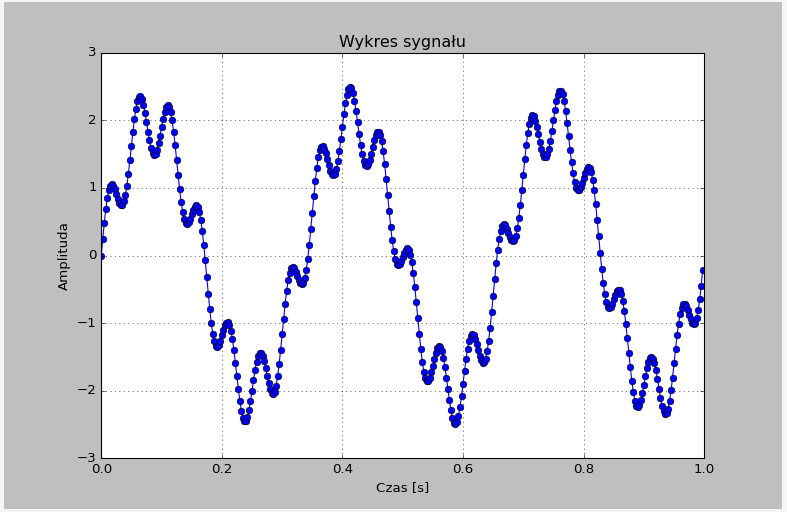
\includegraphics[width=0.7\textwidth]{img/sig.png}
                \caption{Wykres sygnału przed filtracją}
            \end{figure}
            \begin{figure}[h!]
                \centering
                \includegraphics[width=0.7\textwidth]{img/fil15.png}
                \caption{Wykres filtra}
            \end{figure}

            \begin{figure}[h!]
                \centering
                \includegraphics[width=0.7\textwidth]{img/fil16.png}
                \caption{Wykres sygnału po filtracji}
            \end{figure}
            \FloatBarrier
        }
        \newpage

        \subsubsection{Eksperyment 9} {
            \begin{table}[h!]
            \centering
            \begin{tabular}{|l|l|l|l|l|l|}
            \hline
            Typ filtra & Rząd filtra & Częstotliwość odciecia & Typ okna  \\\hline
            Dolnoprzepustowy & 51 & 2 & hamming     \\\hline
            \end{tabular}
            \caption{Parametry filtra}
            \end{table}
            \begin{figure}[h!]
                \centering
                \includegraphics[width=0.7\textwidth]{img/sig.png}
                \caption{Wykres sygnału przed filtracją}
            \end{figure}
            \begin{figure}[h!]
                \centering
                \includegraphics[width=0.7\textwidth]{img/fil17.png}
                \caption{Wykres filtra}
            \end{figure}

            \begin{figure}[h!]
                \centering
                \includegraphics[width=0.7\textwidth]{img/fil18.png}
                \caption{Wykres sygnału po filtracji}
            \end{figure}
            \FloatBarrier
        }
        \newpage

        \subsubsection{Eksperyment 10} {
            \begin{table}[h!]
            \centering
            \begin{tabular}{|l|l|l|l|l|l|}
            \hline
            Typ filtra & Rząd filtra & Częstotliwość odciecia & Typ okna  \\\hline
            Górnoprzepustowy & 51 & 190 & hamming     \\\hline
            \end{tabular}
            \caption{Parametry filtra}
            \end{table}
            \begin{figure}[h!]
                \centering
                \includegraphics[width=0.7\textwidth]{img/sig.png}
                \caption{Wykres sygnału przed filtracją}
            \end{figure}
            \begin{figure}[h!]
                \centering
                \includegraphics[width=0.7\textwidth]{img/fil19.png}
                \caption{Wykres filtra}
            \end{figure}

            \begin{figure}[h!]
                \centering
                \includegraphics[width=0.7\textwidth]{img/fil20.png}
                \caption{Wykres sygnału po filtracji}
            \end{figure}
            \FloatBarrier
        }
        \newpage

        \subsubsection{Eksperyment 11} {
            \begin{table}[h!]
            \centering
            \begin{tabular}{|l|l|l|l|l|l|}
            \hline
            Typ filtra & Rząd filtra & Częstotliwość odciecia & Typ okna  \\\hline
            Górnoprzepustowy & 51 & 195 & hamming     \\\hline
            \end{tabular}
            \caption{Parametry filtra}
            \end{table}
            \begin{figure}[h!]
                \centering
                \includegraphics[width=0.7\textwidth]{img/sig.png}
                \caption{Wykres sygnału przed filtracją}
            \end{figure}
            \begin{figure}[h!]
                \centering
                \includegraphics[width=0.7\textwidth]{img/fil21.png}
                \caption{Wykres filtra}
            \end{figure}

            \begin{figure}[h!]
                \centering
                \includegraphics[width=0.7\textwidth]{img/fil22.png}
                \caption{Wykres sygnału po filtracji}
            \end{figure}
            \FloatBarrier
        }
        \newpage

        \subsubsection{Eksperyment 12} {
            \begin{table}[h!]
            \centering
            \begin{tabular}{|l|l|l|l|l|l|}
            \hline
            Typ filtra & Rząd filtra & Częstotliwość odciecia & Typ okna  \\\hline
            Pasmowy & 51 & 90 & hamming     \\\hline
            \end{tabular}
            \caption{Parametry filtra}
            \end{table}
            \begin{figure}[h!]
                \centering
                \includegraphics[width=0.7\textwidth]{img/sig.png}
                \caption{Wykres sygnału przed filtracją}
            \end{figure}
            \begin{figure}[h!]
                \centering
                \includegraphics[width=0.7\textwidth]{img/fil23.png}
                \caption{Wykres filtra}
            \end{figure}

            \begin{figure}[h!]
                \centering
                \includegraphics[width=0.7\textwidth]{img/fil24.png}
                \caption{Wykres sygnału po filtracji}
            \end{figure}
            \FloatBarrier
        }
        \newpage

        \subsubsection{Eksperyment 13} {
            \begin{table}[h!]
            \centering
            \begin{tabular}{|l|l|l|l|l|l|}
            \hline
            Typ filtra & Rząd filtra & Częstotliwość odciecia & Typ okna  \\\hline
            Pasmowy & 51 & 80 & hamming     \\\hline
            \end{tabular}
            \caption{Parametry filtra}
            \end{table}
            \begin{figure}[h!]
                \centering
                \includegraphics[width=0.7\textwidth]{img/sig.png}
                \caption{Wykres sygnału przed filtracją}
            \end{figure}
            \begin{figure}[h!]
                \centering
                \includegraphics[width=0.7\textwidth]{img/fil25.png}
                \caption{Wykres filtra}
            \end{figure}

            \begin{figure}[h!]
                \centering
                \includegraphics[width=0.7\textwidth]{img/fil26.png}
                \caption{Wykres sygnału po filtracji}
            \end{figure}
            \FloatBarrier
        }
        \newpage
    
    }

    \subsection{Wykorzystanie analizy korelacyjnej do pomiaru odległości} {
        \subsubsection{Eksperyment 1} {
            \begin{table}[h!]
                \centering
                \begin{tabular}{|l|l|l|l|l|}
                    \hline
                    $V_s[m/s]$ & $V_p[m/s]$ & $T_s[s]$ & $f_s[Hz]$ & $l$ \\ \hline
                    100        & 0.5        & 1        & 20        & 60 \\ \hline
                \end{tabular}
                \caption{Parametry wejściowe symulatora}
            \end{table}
            \begin{figure}[h!]
                \centering
                \includegraphics[width=0.8\textwidth]{img/sim1.png}
                \caption{Sygnały w symulatorze czujnika odległości = 6.5}
            \end{figure}
            \begin{figure}[h!]
                \centering
                \includegraphics[width=0.8\textwidth]{img/sim2.png}
                \caption{Sygnały w symulatorze czujnika odległości = 10}
            \end{figure}
            \begin{figure}[h!]
                \centering
                \includegraphics[width=0.8\textwidth]{img/sim3.png}
                \caption{Sygnały w symulatorze czujnika odległości = 12}
            \end{figure}
            \begin{figure}[h!]
                \centering
                \includegraphics[width=0.8\textwidth]{img/sim4.png}
                \caption{Sygnały w symulatorze czujnika odległości = 18.5}
            \end{figure}
            \FloatBarrier
            \begin{table}[h!]
                \centering
                \begin{tabular}{|l|l|l|}
                    \hline
                    $t[s]$ & $d_r[m]$ & $d_m[m]$ \\ \hline
                    06.50  & 3.250    & 2.500    \\ \hline
                    10.00  & 5.000    & 5.000    \\ \hline
                    12.00  & 6.000    & 7.500    \\ \hline
                    18.50  & 9.250    & 10.000    \\ \hline
                \end{tabular}
                \caption{Wyniki działania symulatora}
            \end{table}
        }
        \newpage

        \subsubsection{Eksperyment 2} {
            \begin{table}[h!]
                \centering
                \begin{tabular}{|l|l|l|l|l|}
                    \hline
                    $V_s[m/s]$ & $V_p[m/s]$ & $T_s[s]$ & $f_s[Hz]$ & $l$ \\ \hline
                    1000       & 0.5        & 0.1      & 200       & 40 \\ \hline
                \end{tabular}
                \caption{Parametry wejściowe symulatora}
            \end{table}
            \begin{figure}[h!]
                \centering
                \includegraphics[width=0.8\textwidth]{img/sim5.png}
                \caption{Sygnały w symulatorze czujnika odległości = 1.5}
            \end{figure}
            \begin{figure}[h!]
                \centering
                \includegraphics[width=0.8\textwidth]{img/sim6.png}
                \caption{Sygnały w symulatorze czujnika odległości = 3}
            \end{figure}
            \begin{figure}[h!]
                \centering
                \includegraphics[width=0.8\textwidth]{img/sim7.png}
                \caption{Sygnały w symulatorze czujnika odległości = 6.5}
            \end{figure}
            \begin{figure}[h!]
                \centering
                \includegraphics[width=0.8\textwidth]{img/sim8.png}
                \caption{Sygnały w symulatorze czujnika odległości = 15}
            \end{figure}
            \FloatBarrier
            \begin{table}[h!]
                \centering
                \begin{tabular}{|l|l|l|}
                    \hline
                    $t[s]$ & $d_r[m]$ & $d_m[m]$ \\ \hline
                    01.50  & 0.750    & 0.000    \\ \hline
                    03.00  & 1.500    & 2.500    \\ \hline
                    06.50  & 3.250    & 2.500    \\ \hline
                    15.00  & 7.500    & 7.500    \\ \hline
                \end{tabular}
                \caption{Wyniki działania symulatora}
            \end{table}
        }
        \newpage

        \subsubsection{Eksperyment 3} {
            \begin{table}[h!]
                \centering
                \begin{tabular}{|l|l|l|l|l|}
                    \hline
                    $V_s[m/s]$ & $V_p[m/s]$ & $T_s[s]$ & $f_s[Hz]$ & $l$ \\ \hline
                    1000       & 0.5        & 0.1      & 400       & 40 \\ \hline
                \end{tabular}
                \caption{Parametry wejściowe symulatora}
            \end{table}
            \begin{figure}[h!]
                \centering
                \includegraphics[width=0.8\textwidth]{img/sim9.png}
                \caption{Sygnały w symulatorze czujnika odległości = 1.5}
            \end{figure}
            \begin{figure}[h!]
                \centering
                \includegraphics[width=0.8\textwidth]{img/sim10.png}
                \caption{Sygnały w symulatorze czujnika odległości = 3}
            \end{figure}
            \begin{figure}[h!]
                \centering
                \includegraphics[width=0.8\textwidth]{img/sim11.png}
                \caption{Sygnały w symulatorze czujnika odległości = 7}
            \end{figure}
            \begin{figure}[h!]
                \centering
                \includegraphics[width=0.8\textwidth]{img/sim12.png}
                \caption{Sygnały w symulatorze czujnika odległości = 8.5}
            \end{figure}
            \FloatBarrier
            \begin{table}[h!]
                \centering
                \begin{tabular}{|l|l|l|}
                    \hline
                    $t[s]$ & $d_r[m]$ & $d_m[m]$ \\ \hline
                    01.50  & 0.750    & 1.250    \\ \hline
                    03.00  & 1.500    & 1.250    \\ \hline
                    07.00  & 3.500    & 3.750    \\ \hline
                    08.50  & 4.250    & 5.000    \\ \hline
                \end{tabular}
                \caption{Wyniki działania symulatora}
            \end{table}
        }
        \newpage

        \subsubsection{Eksperyment 4} {
            \begin{table}[h!]
                \centering
                \begin{tabular}{|l|l|l|l|l|}
                    \hline
                    $V_s[m/s]$ & $V_p[m/s]$ & $T_s[s]$ & $f_s[Hz]$ & $l$ \\ \hline
                    1000       & 0.5        & 0.1      & 400       & 20 \\ \hline
                \end{tabular}
                \caption{Parametry wejściowe symulatora}
            \end{table}
            \begin{figure}[h!]
                \centering
                \includegraphics[width=0.8\textwidth]{img/sim13.png}
                \caption{Sygnały w symulatorze czujnika odległości = 1.5}
            \end{figure}
            \begin{figure}[h!]
                \centering
                \includegraphics[width=0.8\textwidth]{img/sim14.png}
                \caption{Sygnały w symulatorze czujnika odległości = 3.5}
            \end{figure}
            \begin{figure}[h!]
                \centering
                \includegraphics[width=0.8\textwidth]{img/sim15.png}
                \caption{Sygnały w symulatorze czujnika odległości = 6}
            \end{figure}
            \begin{figure}[h!]
                \centering
                \includegraphics[width=0.8\textwidth]{img/sim16.png}
                \caption{Sygnały w symulatorze czujnika odległości = 8.5}
            \end{figure}
            \FloatBarrier
            \begin{table}[h!]
                \centering
                \begin{tabular}{|l|l|l|}
                    \hline
                    $t[s]$ & $d_r[m]$ & $d_m[m]$ \\ \hline
                    01.50  & 0.750    & 1.250    \\ \hline
                    03.50  & 1.750    & 1.250    \\ \hline
                    06.00  & 3.000    & 2.500    \\ \hline
                    08.50  & 4.250    & 3.750    \\ \hline
                \end{tabular}
                \caption{Wyniki działania symulatora}
            \end{table}
        }
        \newpage

        \subsubsection{Eksperyment 5} {
            \begin{table}[h!]
                \centering
                \begin{tabular}{|l|l|l|l|l|}
                    \hline
                    $V_s[m/s]$ & $V_p[m/s]$ & $T_s[s]$ & $f_s[Hz]$ & $l$ \\ \hline
                    100        & 3.0        & 1        & 20        & 20 \\ \hline
                \end{tabular}
                \caption{Parametry wejściowe symulatora}
            \end{table}
            \begin{figure}[h!]
                \centering
                \includegraphics[width=0.8\textwidth]{img/sim17.png}
                \caption{Sygnały w symulatorze czujnika odległości = 1.5}
            \end{figure}
            \begin{figure}[h!]
                \centering
                \includegraphics[width=0.8\textwidth]{img/sim18.png}
                \caption{Sygnały w symulatorze czujnika odległości = 3}
            \end{figure}
            \begin{figure}[h!]
                \centering
                \includegraphics[width=0.8\textwidth]{img/sim19.png}
                \caption{Sygnały w symulatorze czujnika odległości = 4.5}
            \end{figure}
            \begin{figure}[h!]
                \centering
                \includegraphics[width=0.8\textwidth]{img/sim20.png}
                \caption{Sygnały w symulatorze czujnika odległości = 10}
            \end{figure}
            \FloatBarrier
            \begin{table}[h!]
                \centering
                \begin{tabular}{|l|l|l|}
                    \hline
                    $t[s]$ & $d_r[m]$ & $d_m[m]$ \\ \hline
                    01.50  & 4.500    & 5.000    \\ \hline
                    03.00  & 9.000    & 10.000    \\ \hline
                    04.50  & 13.500   & 15.000    \\ \hline
                    10.00  & 27.500   & 30.000    \\ \hline
                \end{tabular}
                \caption{Wyniki działania symulatora}
            \end{table}
        }
        \newpage
    }
\section{Dyskusja}

    \subsection{Splot i korelacja sygnałów dyskretnych} {
        Pierwsza wykonana seria eksperymentów jest poświęcona operacji splotu i
        korelacji sygnałów dykretnych, które to operacje należało zaimplementować w
        ramach wykonywanego zadania. Eksperymenty od \ref{eksperyment:splot1} do
        \ref{eksperyment:splot3} prezentują wyniki operacji splotu, a eksperymenty od
        \ref{eksperyment:korelacja1} do \ref{eksperyment:korelacja3} wyniki operacji
        korelacji. Dokumentacja każdego pojedynczego doświadczenia zawiera wykresy
        oraz parametry dwóch sygnałów na których operacja została wykonana, a także
        wykres sygnału wynikowego. W pierwszym doświadczenie \ref{eksperyment:splot1}
        wykorzystano dwa praktycznie takie same sygnały sinusoidalne, różniące się
        jedynie momentem rozpoczęcia, który to parametr nie ma wpływu na wynik
        splotu. Można więc uznać że wykonano splot dwóch takich samych sygnałów
        sinusoidalnych. Symetryczny kształt sygnału wynikowego wskazuje na to, że
        rzeczywiście sygnały wejścioweg były takie same. Ciekawe okazuje się
        porównanie z wynikami doświadczenia \ref{eksperyment:korelacja1}, w którym to
        te same sygnały zostały ze sobą skorelowane. Wynik tego eksperymenty jest
        odbiciem lustrzanym eksperymenty \ref{eksperyment:splot1} względem osi czasu,
        co wskazuje na pewne podobieństwo i związek między operacją splotu i korelacji
        sygnałów. W doświadczeniach \ref{eksperyment:splot2} i
        \ref{eksperyment:korelacja2} wykorzystano parę funkcji sinus i sinus
        wyprostowany jednopołówkowo. Wynik okazuje się w obu doświadczeniach bardzo
        podobny. Tym razem jednak odkrywamy, że jest to odbicie symetryczne nie tylko
        względem osi poziomej, ale również osi pionowej, czego ze względu na symetrię
        wykresu nie dało się zauważyć w poprzednio omawianej parze doświadczeń. W
        ostatniej parze eksperymentów \ref{eksperyment:splot3} oraz
        \ref{eksperyment:korelacja3} wykorzystano połączenie funkcji sinus z funkcją
        trójkątną. Wynik jest wizualnie ciekawy, w stosunku do wyników poprzednich.
        Okazuje się praktycznie identyczny dla splotu i korelacji ze względu na to,
        iż jest symetryczny względem swojego środka.
    }

    \subsection{Filtracja sygnałów dyskretnych} {
        Druga grupa eksperymentów poświęcona jest filtrom o skończonej odpowiedzi
        impulsowej. Na początku wygenerowany został sygnał przeznaczony do filtrowania,
        jak opisano w \ref{metody:filtracja}. Następnie w każdym kolejnym eksperymencie
        utworzony został nowy filtr, na którym wykonano splot ze wspomnianym wcześniej
        sygnałem złożonym. Dla każdego doświadczenia zaprezentowano wykres i parametry
        filtru oraz wykres sygnału po filtracji. Warto jeszcze przed analizą wyników
        zauważyć, że filtrowany sygnał posiada dwie, dające się wizualnie wyróżnić
        składowe, jedna o częstotliwości $20Hz$ a druga o częstotliwości $3Hz$.

        Pierwsze cztery eksperymenty poświęcone są badaniu wpływu wybranej funkcji
        okna na jakość filtracji. Tak więc kolejno zastosowane zostały okno
        kwadratowe, okno hamminga, okno hanninga i okno blackmana. W każdym przypadku
        wykorzystanu tutaj filtr dolnoprzepustowy rzędu 51 i częstotliwość odcięcia
        $5Hz$. Doświadczalnie stwierdzono, że przy tych parametrach różnica w
        wykorzystaniu okien staje się widoczna. I tak dla wspomnianych parametrów
        wizualnie daje się stwierdzić, że najlepszą jakość filtracji osiągnięto dla
        okna hammina, a najgorszą dla okna kwadratowego. Przy czym wyniki dla okna
        hanninga i hamminga niewiele się różnią, przy oknie blackmana daje się
        zauważyć, że jakaś inna częstotliwość składowa kiedyś istniała. Natomiast w
        przypadku okna prostokątnego składowa o wyższej częstotliwości wyraźnie się
        zaznacza. Warto jednak wspomnieć, że w każdym przypadku udało się tą wyższą
        składową wyraźnie lub całkowicie wytłumić.

        Kolejne trzy eksperymenty pokazują wpływ rzędu filtra (liczby jego próbek) na
        jakość filtrowania. Każdorazowo wykorzystano tutaj również filtr
        dolnoprzepustowy, czestotliwość odcięcia $5Hz$ i okno hammina. Wyniki okazują
        się zgodne z intuicją. Czym większy rząd filtra tym silniej udaje się wytłumić
        częstotliwość $20Hz$. Za pierwszym razem (rząd 41) wyższa składowa wytłumiona
        zostaje praktycznie całkowicie. Za drugim razem jest wyraźnie zauważalna, choć
        słabsza niż w sygnale oryginalnym. Wynik trzeciego doświadczenia (rząd 21)
        wizualnie niewiele różni się od sygnału filtrowanego.

        W ostatniej serii doświadczeń (od 8 do 13) wykorzystane zostały różne
        częstotliwości odcięcia jak i różne typy filtrów. W eksperymentach 8 i 9
        zastosowano częstotliwość odcięcia mniejszą i równą najniższej częstotliwości
        składowej sygnału, przy wykorzystaniu filtru dolnoprzepustowego. W wyniku
        wyższa składowa została wytłumiona całkowicie a niższa odpowiednio dla wyższej
        częstotliwości odcięcia - wytłumiona słabiej, natomiast dla niższej
        częstotliwości odcięcia - wytłumiona silniej. Odfiltrowywana była bowiem
        czestotliwośc niższa, a pozostawiona częstotliwość wyższa - $20Hz$. W
        eksperymencie 10 zastosowano filtr górnoprzepustowy a częstotliwość odcięcia
        $f_o$ wynosiła 190, co dla tego filtru przekłada się na częstotliwość $f_{o2} =
        200Hz / 2 - 190Hz = 10Hz$. Na wykresie wynikowym widać, że faktycznie
        częstotliwość $3Hz$ została prawie całkowicie wytłumiona, da się jednak
        zauważyć jej obecność w nieznacznych "wahaniach" całego wykresu w góre i w
        dół. Przy zastosowaniu częstotliwości odcięcia $f_o = 195Hz$ dla tego samego
        filtra, wspomniana niższa częstotliwość zaznacza się znacznie wyraźniej. W obu
        przypadkach można jednak spokojnie stwierdzić, że składowa niższa jest
        słabsza niż składowa wyższa. Ostatnie dwa eksperymenty wykonano za pomocą
        filtra pasmowoprzepustowego, ustawiono częstotliwość odcięcia $f_o = 90Hz$, co
        dla tego filtra oznacza, że pasmo przepustowe mieściło się między $10Hz$ a
        $190$ Hz. W pierwszym z dwóch eksperymentów niższa częstotliwość została
        prawie całkowicie wytłumiona. W ostatnim przypadku częstotliwość niższa
        została wytłumiona tak, że nie jest już zauważalna na wykresie.
    }

    \subsection{Wykorzystanie analizy korelacyjnej do pomiaru odległości} {
        Ostatnia część eksperymentów została poświęcona badaniu zachowania
        korelacyjnego czujnika odległości. Dla każdego eksperymentu zostały
        przedstawione parametry wejściowe symulatora, wykresy sygnałów sondującego,
        powrotnego i ich korelacji oraz kilka pomiarów czujnika razem z rzeczywistymi
        odległościami. Pierwszy eksperyment został przeprowadzony dla prędkości
        sygnału $100m/s$ i odległości do przedmiotu około $30m$. Przedmiot oddala się
        nieznacznie z prędkością $0.5m/s$. Okres sygnału sondującego wynosi $1s$.
        Próbek w buforze jest $60$, co przy częstotliwości próbkowania $20Hz$ oznacza
        trzy pełne okresy. Okaże się, czy jest potrzeba przechowywać tyle próbek. Po
        przyjrzeniu się wynikom widać, że najogólniej mówiąc czujnik działa poprawnie,
        natomiast ma ograniczoną dokładność pomiaru do ok $2.5m$. Dokładność ta może
        być zadowalająca lub nie, w zależności od wymagań czujnika.

        \paragraph{Zakres działania czujnika} jest pierwszą rzeczą, na którą warto
        zwrócić uwagę. Można zastanowić się co ma na ten zakres decydujący wpływ.
        Rozważmy prędkość sygnału. Kolejny eksperyment (2) pokazuje, że sama prędkość
        nie wpływa w żaden sposób na dokładność pomiaru, gdyż przy prędkości $1000m/s$
        uzyskaliśmy tę samą dokładność, co przy prędkości $100m/s$. Ważny jest
        natomiast stosunek prędkości do okresu sygnału. Okres sygnału sondującego
        wyznacza zakres opóźnień, sygnału powrotnego, dla których uda się poprawnie
        obliczyć odległość. W idealnym przypadku, opóźnienie musi być oczywiście
        mniejsze niż okres, bo przy analizie korelacyjnej nie będzie się dało w żaden
        sposób stwierdzić, czy sygnał powrotny jest opóźniony o $kT + x$, czy tylko o
        $x$, gdzie $kT$ to dowolna całkowita wieloktrotność okresu a $x$ to pewne
        opóźnienie sygnału. W praktyce granica ta zależy od jeszcze wielu innych
        czynnników, jak charakterystyka samego sygnału sondującego oraz liczba okresów
        sygnału przechowywana w buforze. W eksperymencie 5 okazało się, że już gdy
        opóźnienie stało się większe niż ok $0.4$ część okresu, to czujnik nie był w
        stanie określić faktycznej odległości i zaczął znowu "od zera". Ostateczny
        wniosek jest więc taki, że na zakres działania czujnika ma wpływ stosunek
        prędkości sygnału sondującego do jego okresu. Sam okres wyznacza zakres
        opóźnień a prędkość decyduje o tym, jaki zakres odległości będzie odpowiadał
        danemu zakresowi opóźnień.

        \paragraph{Dokładność działania czujnika} zależy w decydującej mierze od
        częstotliwości próbkowania. A dokładnie nie od samej bezwzględnej wartości
        częstotliwości ale od liczby próbek przypadającej na okres. Czym więcej próbek
        na okres tym z większą dokładnością można stwierdzić, jakie jest opóźnienie
        sygnału powrotnego. Eksperyment 3 pokazuje, że po zwiększeniu częstotliwości
        próbkowania (co skutkowało zwiększeniem liczby próbek przypadających na okres
        sygnału), uzyskalismy większą dokładność niż w eksperymencie 2. Zostaje
        jeszcze do rozważenia ostatni parametr, a mianowicie długość bufora, którą od
        razu możemy przełożyć na faktycznie mającą znaczenie - liczbę okresów sygnału
        w buforze. Wartość ta jest bardzo istotna i eksperyment 4 pokazuje, że jeżeli
        będzie zbyt mała, to po prostu czujnik przestanie działać, gdyż analiza
        korelacyjna nie wykaże żadnego lokalnego maksimum korelacji. Pojawia się
        pytanie jaka powinna być wartość tego parametru. Oczywiście chcielibyśmy, żeby
        była jak najmniejsza, ponieważ czym mniej próbek w buforze, tym szybciej można
        przeprowadzić obliczenia, a czym szybciej znajdujemy wynik korelacji tym
        większą częstotliwość próbkowania możemy uzyskać, co w konsekwencji skutkuje
        większą dokładnością czujnika. W eksperymentach 1, 2 i 3 kolejno wartość ta
        była zmniejszana od trzykrotności okresu do pojedynczego okresu sygnału
        sondującego. Za żadnym razem zmniejszenie tej wartości nie wpłynęło negatywnie
        na analizę korelacyjną. Można więc na podstawie doświadczeń stwierdzić, że
        wystarczy w buforze przechowywać jeden okres. Okazuje się jednak, że nie jest
        to zasada, gdyż przy zastosowaniu mniej złożonej funkcji (np. czysty sinus),
        wartość ta była już za mała (niestety nie udokumentowano tego w tym
        sprawozdaniu). Można więc wysnuć wniosek, że charakter funkcji sondującej
        jest bardzo istotny, ponieważ od kształtu tej funkcji zależy, jaką minimalną
        wielokrotność (lub część) okresów trzeba przechować w buforze, aby poddana
        analizie korelacyjnej dała poprawne wyniki. Jak już wcześniej wspomniano, ma
        to decydujący wpływ na dokładność pomiaru.
    }

\section{Wnioski} {
    \begin{itemize}
        \item Operacje splotu i korelacji sygnałów dyskretnych są do siebie bardzo
            zbliżone
        \item Okno prostokątne najgorzej wpływa na jakość filtracji sygnału
        \item Czym większy rząd filtra tym lepsza jakość filtracji
        \item Jeżeli pasmo przepustowe nie obejmuje żadnej składowej to wszystkie
            składowe są tłumione, tym bardziej, im dalej znajdują się od granicy pasma
            przepustowego
        \item Korelacyjny czujnik odległości ma ograniczony zakres pomiaru wyznaczony
            przez stosunek prędkości sygnału sondującego do okresu tego sygnału
        \item Dokładność pomiaru korelacyjnego czujnika odległości jest zdeterminowana
            przez liczbę próbek przypadającą na jeden okres
        \item Charakterystyka sygnału sondującego ma duże znaczenie zarówno dla
            zakresu pomiaru czujnika korelacyjnego (charakterystyka wyniku korelacji),
            jak i dla dokładności pomiaru (minimalna długość bufora potrzebna do
            uzyskania poprawnego wyniku)
    \end{itemize}
}

%%%%%%%%%%%%%%%%%%%%%%%%%%%%%%%%%%%%%%%%%%%%%%%%%%%%%%%%%%%%%%%%%%%%%%%%%%%%%%%%%%%%%%%%%%%%%%%%%%%%%%%%%%%%%%%%%
% BIBLIOGRAFIA
%%%%%%%%%%%%%%%%%%%%%%%%%%%%%%%%%%%%%%%%%%%%%%%%%%%%%%%%%%%%%%%%%%%%%%%%%%%%%%%%%%%%%%%%%%%%%%%%%%%%%%%%%%%%%%%%%

\begin{thebibliography}{9}

    \bibitem{instrukcja}
    Politechnika Łódzka, 
    \emph{Instrukcja do zadania 3}, 
    Dostęp online: \url{https://ftims.edu.p.lodz.pl/mod/url/view.php?id=6495}, 
    [dostęp: 10 maja 2025].


    \bibitem{python-doc}
    Python Software Foundation, 
    \emph{Python Documentation}, 
    Dostęp online: \url{https://docs.python.org/3/}, 
    [dostęp: 10 maja 2025].

    \bibitem{tkinter-doc}
    Python Software Foundation, 
    \emph{Tkinter Documentation}, 
    Dostęp online: \url{https://docs.python.org/3/library/tkinter.html}, 
    [dostęp: 10 maja 2025].

\end{thebibliography}

\end{document}
